% !TeX root = 00-main.tex
% Results chapter -- CRRT-UDE / StageBridge

\chapter{Results}
\label{chap:results}

Niche-conditioned regulatory transport, and the context-residual estimand $R_{\text{cond}}$ defined in Chapter~\ref{chap:methods}, were estimated on the epithelial compartment of the LUAD progression series and, as a cross-disease calibration probe, on a graded pancreatic intraepithelial neoplasia (PanIN) series.

\section{The progression series is edge-supported by shared donors at every step except the invasion boundary}
\label{sec:cohort}

The LUAD atlas spans the five morphological stages defined in Section~\ref{sec:methods-cohorts}, from Normal through AAH, AIS, and MIA to invasive LUAD. Donor coverage per stage is 23 Normal, 10 AAH, 12 AIS, 4 MIA, and 25 LUAD donors. Because niche-conditioned transport was estimated between adjacent stages, the operative quantity is the number of donors that contribute epithelium to \emph{both} ends of an edge, which sets how much of each estimate is anchored within-patient rather than across-patient (Table~\ref{tab:edge_support}). The early edges are supported: eight donors bridge Normal$\rightarrow$AAH and two bridge AAH$\rightarrow$AIS. The invasion boundary AIS$\rightarrow$MIA has zero shared donors, so any transport across it is necessarily estimated across patients, whereas MIA$\rightarrow$LUAD recovers four shared donors. The AAH$\rightarrow$AIS edge, on which the primary regulatory analysis was run, carries 29{,}712 AAH epithelial receivers and 48{,}688 AIS epithelial cells. (Fig.~\ref{fig:cohort_umap})

\begin{figure}[htbp]
  \centering
  \begin{subfigure}{0.62\textwidth}
    \centering
    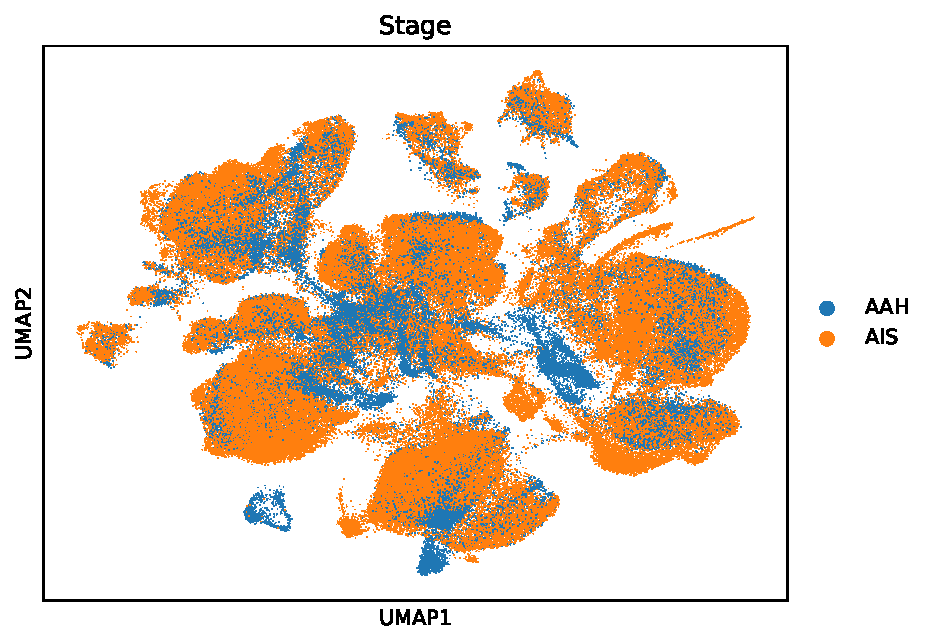
\includegraphics[width=\textwidth]{figures/embeddings/cohort_umap_stage_AAH_AIS.pdf}
    \caption{Colored by progression stage (AAH, AIS)}
    \label{fig:cohort_umap_stage}
  \end{subfigure}

  \vspace{0.6em}

  \begin{subfigure}{\textwidth}
    \centering
    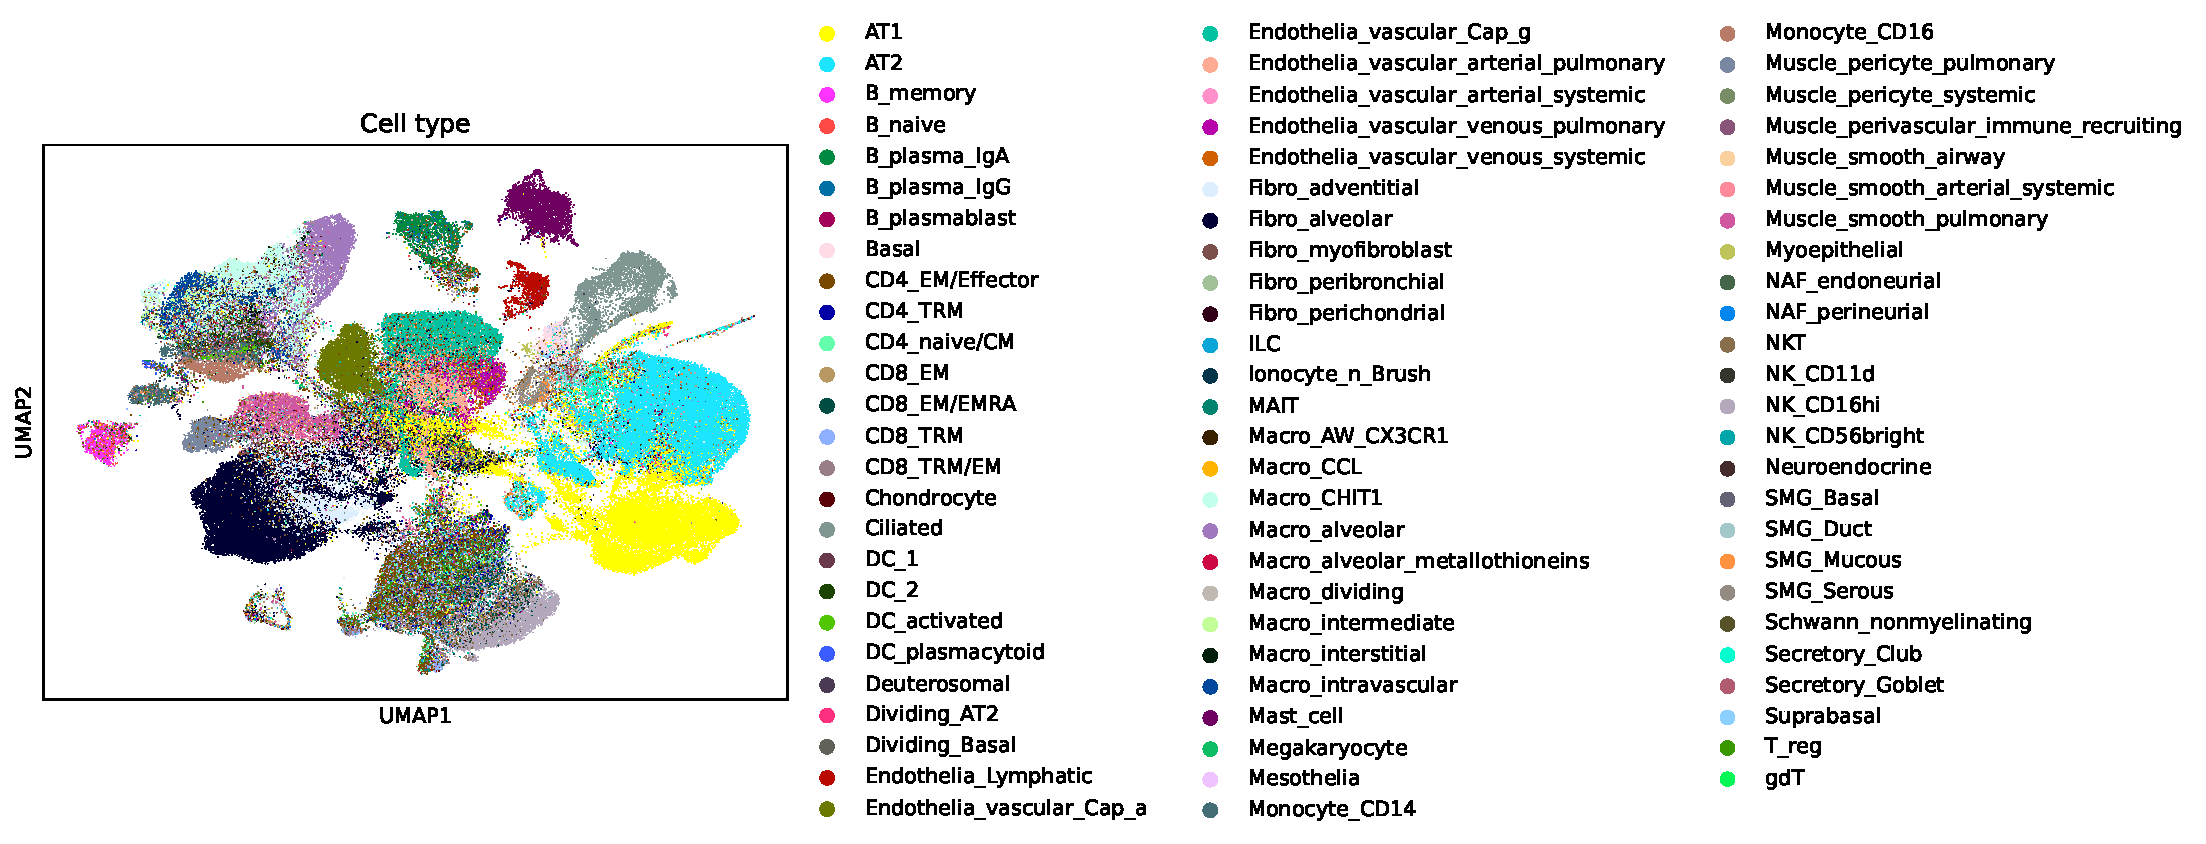
\includegraphics[width=\textwidth]{figures/embeddings/cohort_umap_celltype_AAH_AIS.pdf}
    \caption{Colored by cell-type annotation}
    \label{fig:cohort_umap_celltype}
  \end{subfigure}
  \caption[Single-cell UMAP of the AAH$\rightarrow$AIS cohort]{UMAP of the single-cell transcriptomes
  in the AAH$\rightarrow$AIS cohort, the edge carrying the primary analysis. \textbf{(a)}~By stage: AAH
  (blue) and AIS (orange) overlap broadly, so the stages are not separable by embedding position alone.
  \textbf{(b)}~By fine cell type, spanning epithelial, immune, stromal, and endothelial compartments;
  the epithelial \emph{receivers} entering transport ($29{,}712$ AAH, $48{,}688$ AIS) come from the
  epithelial populations here. The subtle whole-transcriptome stage distinction motivates the
  program-resolved transport estimand over a raw embedding contrast.}
  \label{fig:cohort_umap}
\end{figure}


\begin{table}[htbp]
  \centering
  \caption[Edge support across the LUAD progression ladder]{Edge support across the LUAD progression ladder. Shared donors are those contributing epithelium to both the source and target stage of an edge; they set the within-patient anchoring available to each transport estimate. The AIS$\rightarrow$MIA invasion boundary has no shared donors.}
  \label{tab:edge_support}
  \begin{tabular}{lcccc}
    \toprule
    Edge & Source donors & Target donors & Shared donors & Target epi.\ cells \\
    \midrule
    Normal $\rightarrow$ AAH & 23 & 10 & 8 & 29{,}712 \\
    AAH $\rightarrow$ AIS     & 10 & 12 & 2 & 48{,}688 \\
    AIS $\rightarrow$ MIA     & 12 & 4  & 0 & 8{,}356 \\
    MIA $\rightarrow$ LUAD    & 4  & 25 & 4 & 144{,}226 \\
    \bottomrule
  \end{tabular}
\end{table}

\section{A conditional-stratified coupling is the only estimand that clears the frozen identifiability benchmark}
\label{sec:results-estimand}

Three candidate estimands---a conditional-stratified coupling, a strict $z$-standardized coupling, and a progression-geometry coupling---were screened against a frozen identifiability benchmark with two tiers and four fixed bars: recovery cosine $\geq 0.80$, seed-direction agreement $\geq 0.90$, null gain $< 0.10$, and non-identifiable correlation $< 0.50$. The conditional-stratified coupling passed both tiers and was selected. The strict $z$ coupling passed Tier-1 but failed Tier-2, and the progression-geometry coupling failed both tiers. All downstream regulatory results are therefore reported under the conditional-stratified estimand, which is the single candidate identifiable against the benchmark; the two rejected couplings are retained only as falsification-ladder rungs (Section~\ref{sec:results-ladder}).

\section{The context representation does not encode receiver state}
\label{sec:leakage}

A separate ladder rung audits the estimand for circularity directly: if the context vector $w$ encoded a disguised copy of the receiver's own state $z$, any context effect would be self-referential. A ridge regressor fit from $w$ to $z$ on training receivers and evaluated on held-out receivers cannot reconstruct receiver state---the held-out $R^2$ is negative in every one of the five folds (mean $-0.54$, range $-0.22$ to $-1.03$), i.e.\ $w$ predicts $z$ worse than the mean out of sample. True context does reduce reconstruction error relative to a shuffled control (mean reconstruction MSE $0.48$ versus $0.82$), indicating that $w$ carries some state-correlated information---expected, since tissue ecology and epithelial state are biologically correlated---but both fail to recover receiver state out of sample. The context representation therefore does not carry receiver identity, and the context effect is not an artifact of leakage.

\section{Twenty-nine regulatory programs are stably niche-redirected across the preinvasive AAH$\rightarrow$AIS edge}
\label{sec:stable}

Per-program conditional regulatory transport, $R_{\text{cond}}$, was estimated on the AAH$\rightarrow$AIS edge across five patient-held-out folds for 773 regulatory programs. Twenty-nine programs are STABLE---their held-out $R_{\text{cond}}$ confidence interval excludes zero and holds sign in every fold---30 are DIRECTIONALLY\_STABLE, and 714 are UNSTABLE (Fig.~\ref{fig:forest}). The stable set is a $3.8\%$ minority of the 773 programs. Requiring the effect to survive independently in all five folds, rather than a per-program false-discovery correction on a single-pass $P$ value, is the multiple-comparison control used here, and it is stricter than an FDR threshold on pooled estimates because a program must clear the bar five times on disjoint patient sets. The confirmatory retrained-shuffle null (Section~\ref{sec:hypothesis-assessment}) is the complementary test still outstanding.

The stable programs define a proliferative and stress-response axis. Among PROGENy pathway programs, three are stable and all are context-upregulated: p53 (mean $R_{\text{cond}}$ $+0.295$; 95\% CI, $+0.246$ to $+0.344$), WNT ($+0.293$; $+0.255$ to $+0.331$), and TRAIL ($+0.203$; $+0.184$ to $+0.221$). EGFR is directionally stable and upregulated ($+0.308$; 95\% CI, $+0.280$ to $+0.336$), and JAK-STAT is directionally stable and downregulated ($-0.246$; $-0.313$ to $-0.179$). The stable transcription factors partition into a context-upregulated set led by the AP-1 factor FOS ($+0.141$; $+0.124$ to $+0.157$), together with KAT5 ($+0.127$), PAX8 ($+0.118$), and RB1 ($+0.110$), and a context-downregulated set comprising ZBTB18 ($-0.140$), GLI3 ($-0.129$), the interferon regulator IRF9 ($-0.129$), ETV3 ($-0.126$), ETV6 ($-0.106$), and SMAD4 ($-0.099$). The pattern is a coordinated upregulation of p53, WNT, TRAIL, and AP-1 activity coupled to a downregulation of interferon (IRF9) and TGF$\beta$-effector (SMAD4) signaling, associated with the AAH-to-AIS transition rather than reflecting a stage-averaged shift.

These stable programs establish that a reproducible, sign-consistent, program-level context residual exists under patient-held-out resampling. Whether this reproducible set also exceeds a retrained shuffled-context baseline at the estimand level is a stronger test, deferred to Section~\ref{sec:hypothesis-assessment}. Whether that residual reflects information carried by \emph{local}, cell-resolved niche identity---as opposed to coarser, specimen-level ecology---is a further and stronger question, and the falsification ladder of Section~\ref{sec:results-ladder} answers it in the negative. The ecological reason for that boundary is developed in Section~\ref{sec:results-scale}.

\begin{figure}[htbp]
  \centering
  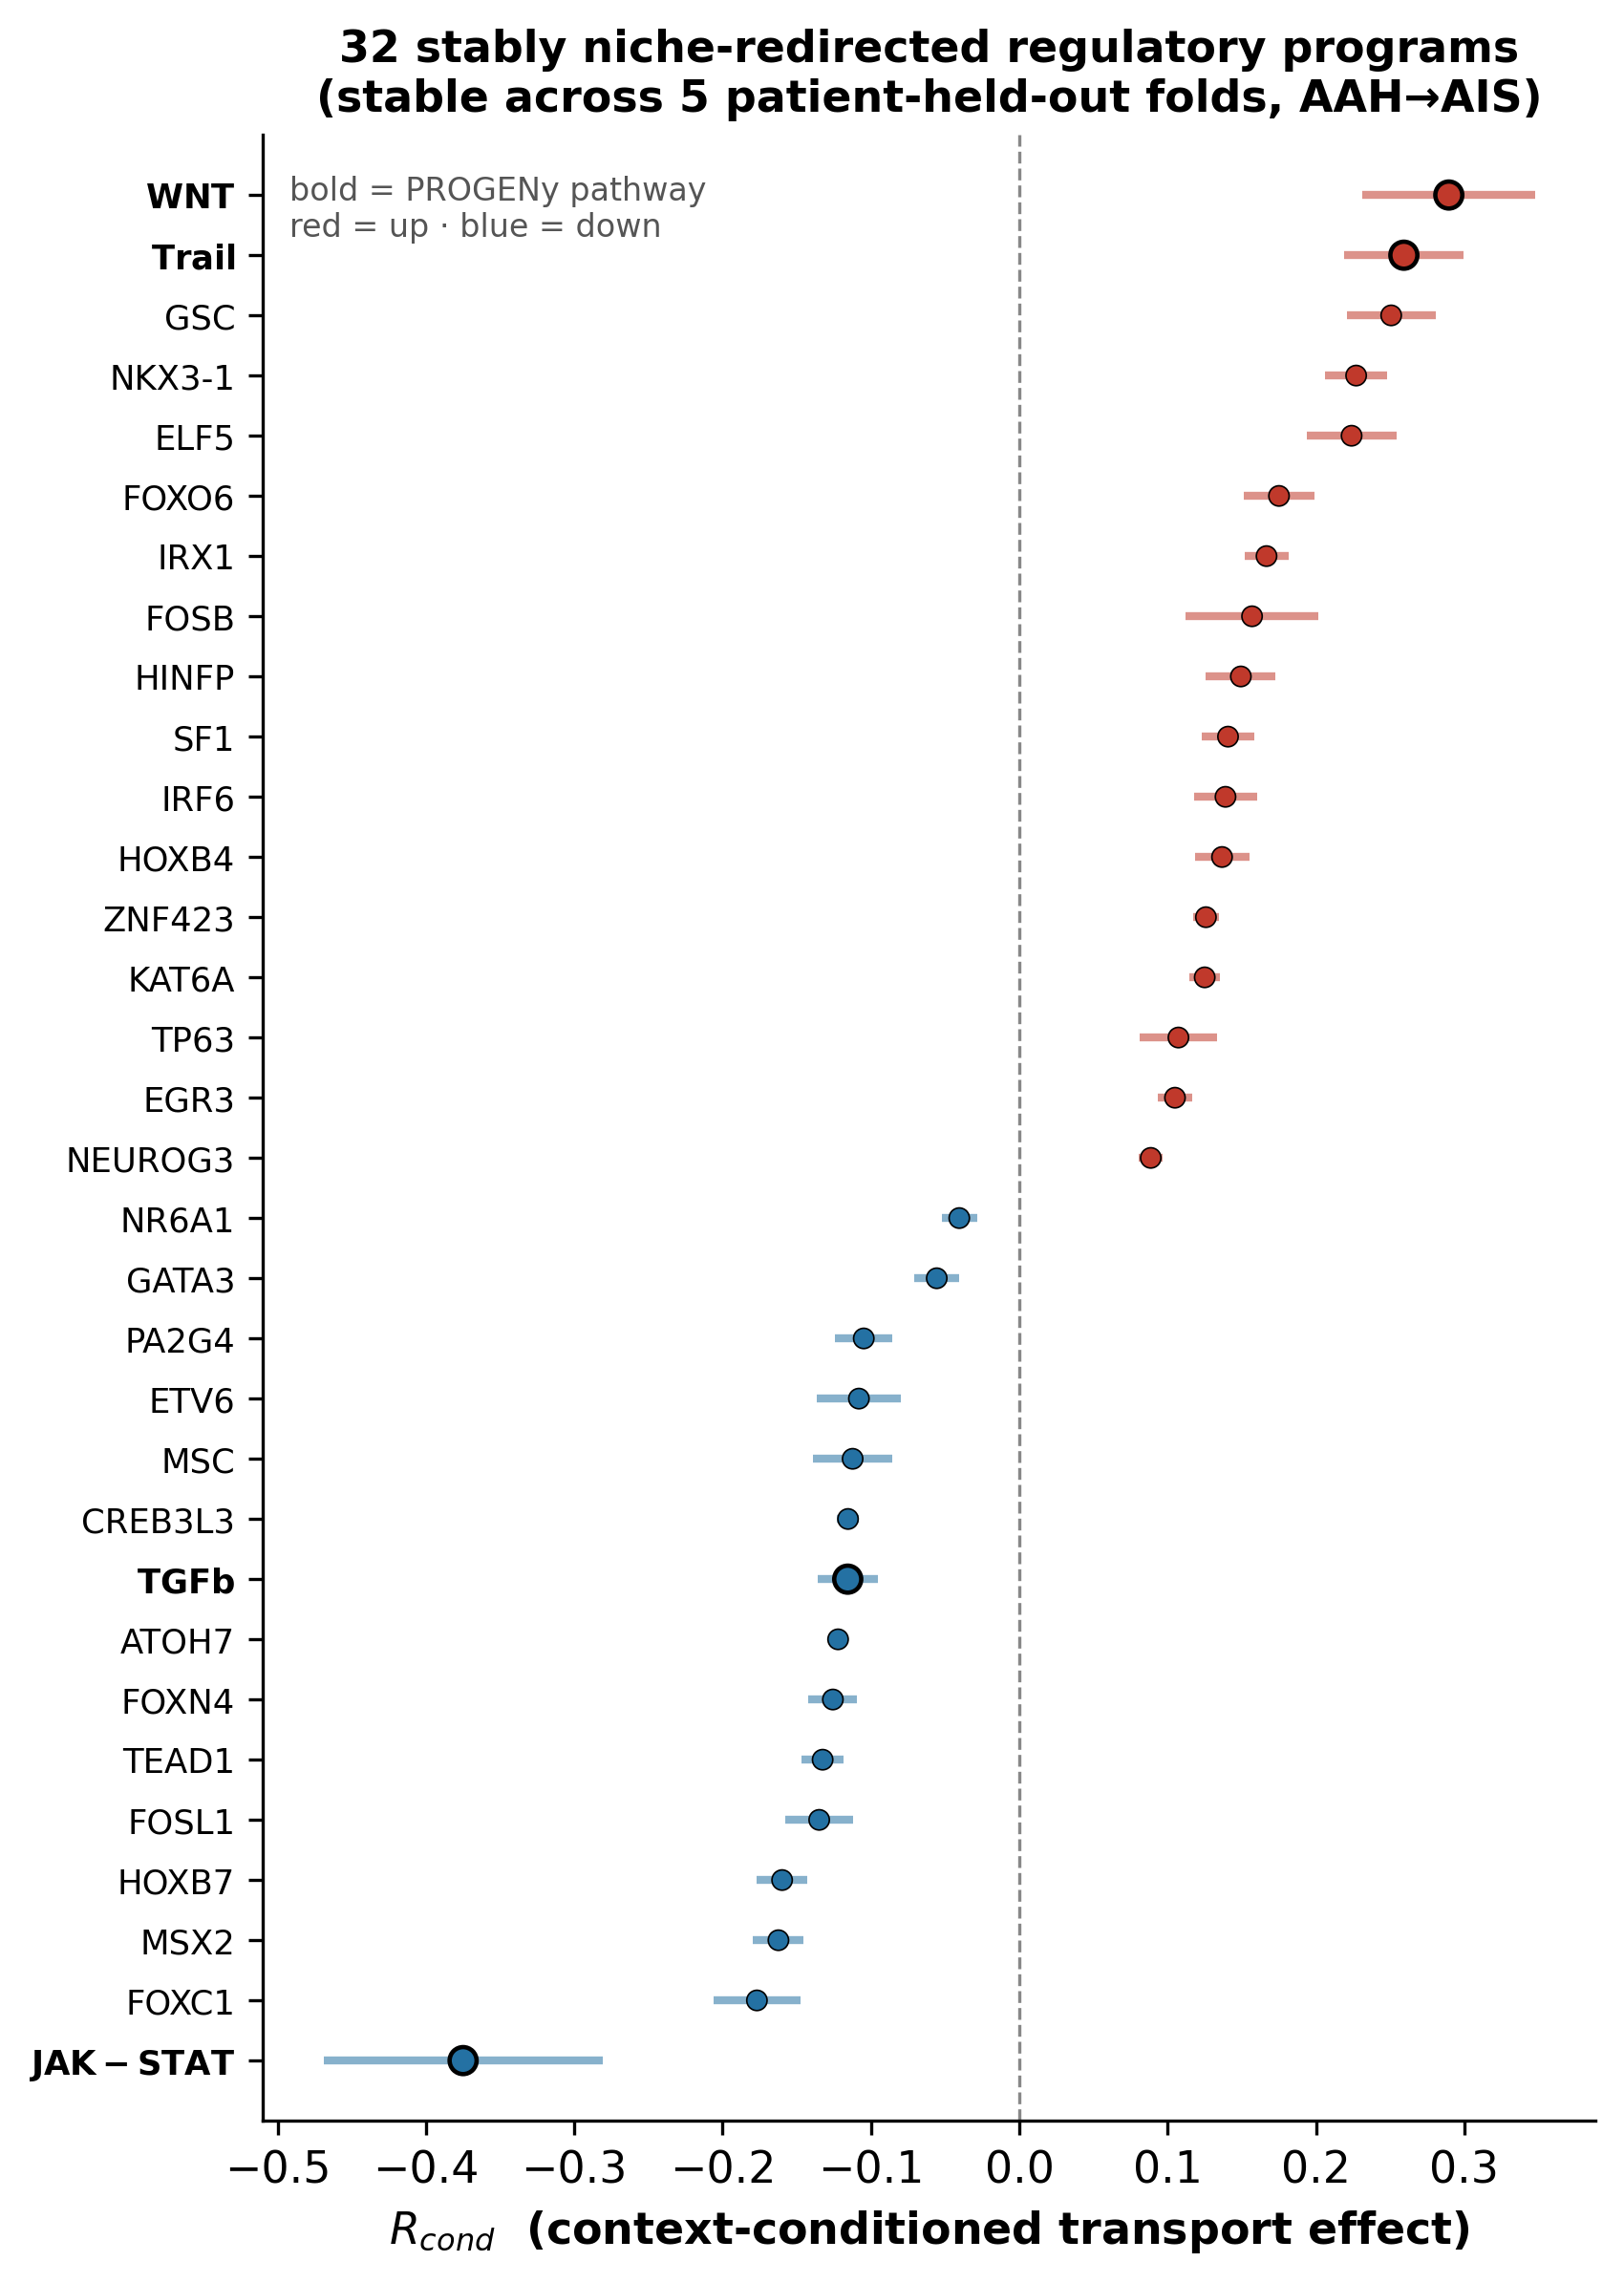
\includegraphics[width=0.9\textwidth]{figures/fig_stable_programs_forest.png}
  \caption[Stable niche-redirected regulatory programs on the AAH$\rightarrow$AIS edge]{The stably niche-redirected regulatory programs on the AAH$\rightarrow$AIS edge. Points are mean conditional transport $R_{\text{cond}}$ over five patient-held-out folds; bars are held-out confidence intervals. Programs are classed STABLE only when the interval excludes zero and holds sign in all folds. p53, WNT, TRAIL, and the AP-1 factor FOS gain context weight; interferon (IRF9) and the TGF$\beta$ effector SMAD4 lose it.}
  \label{fig:forest}
\end{figure}

\begin{figure}[htbp]
  \centering
  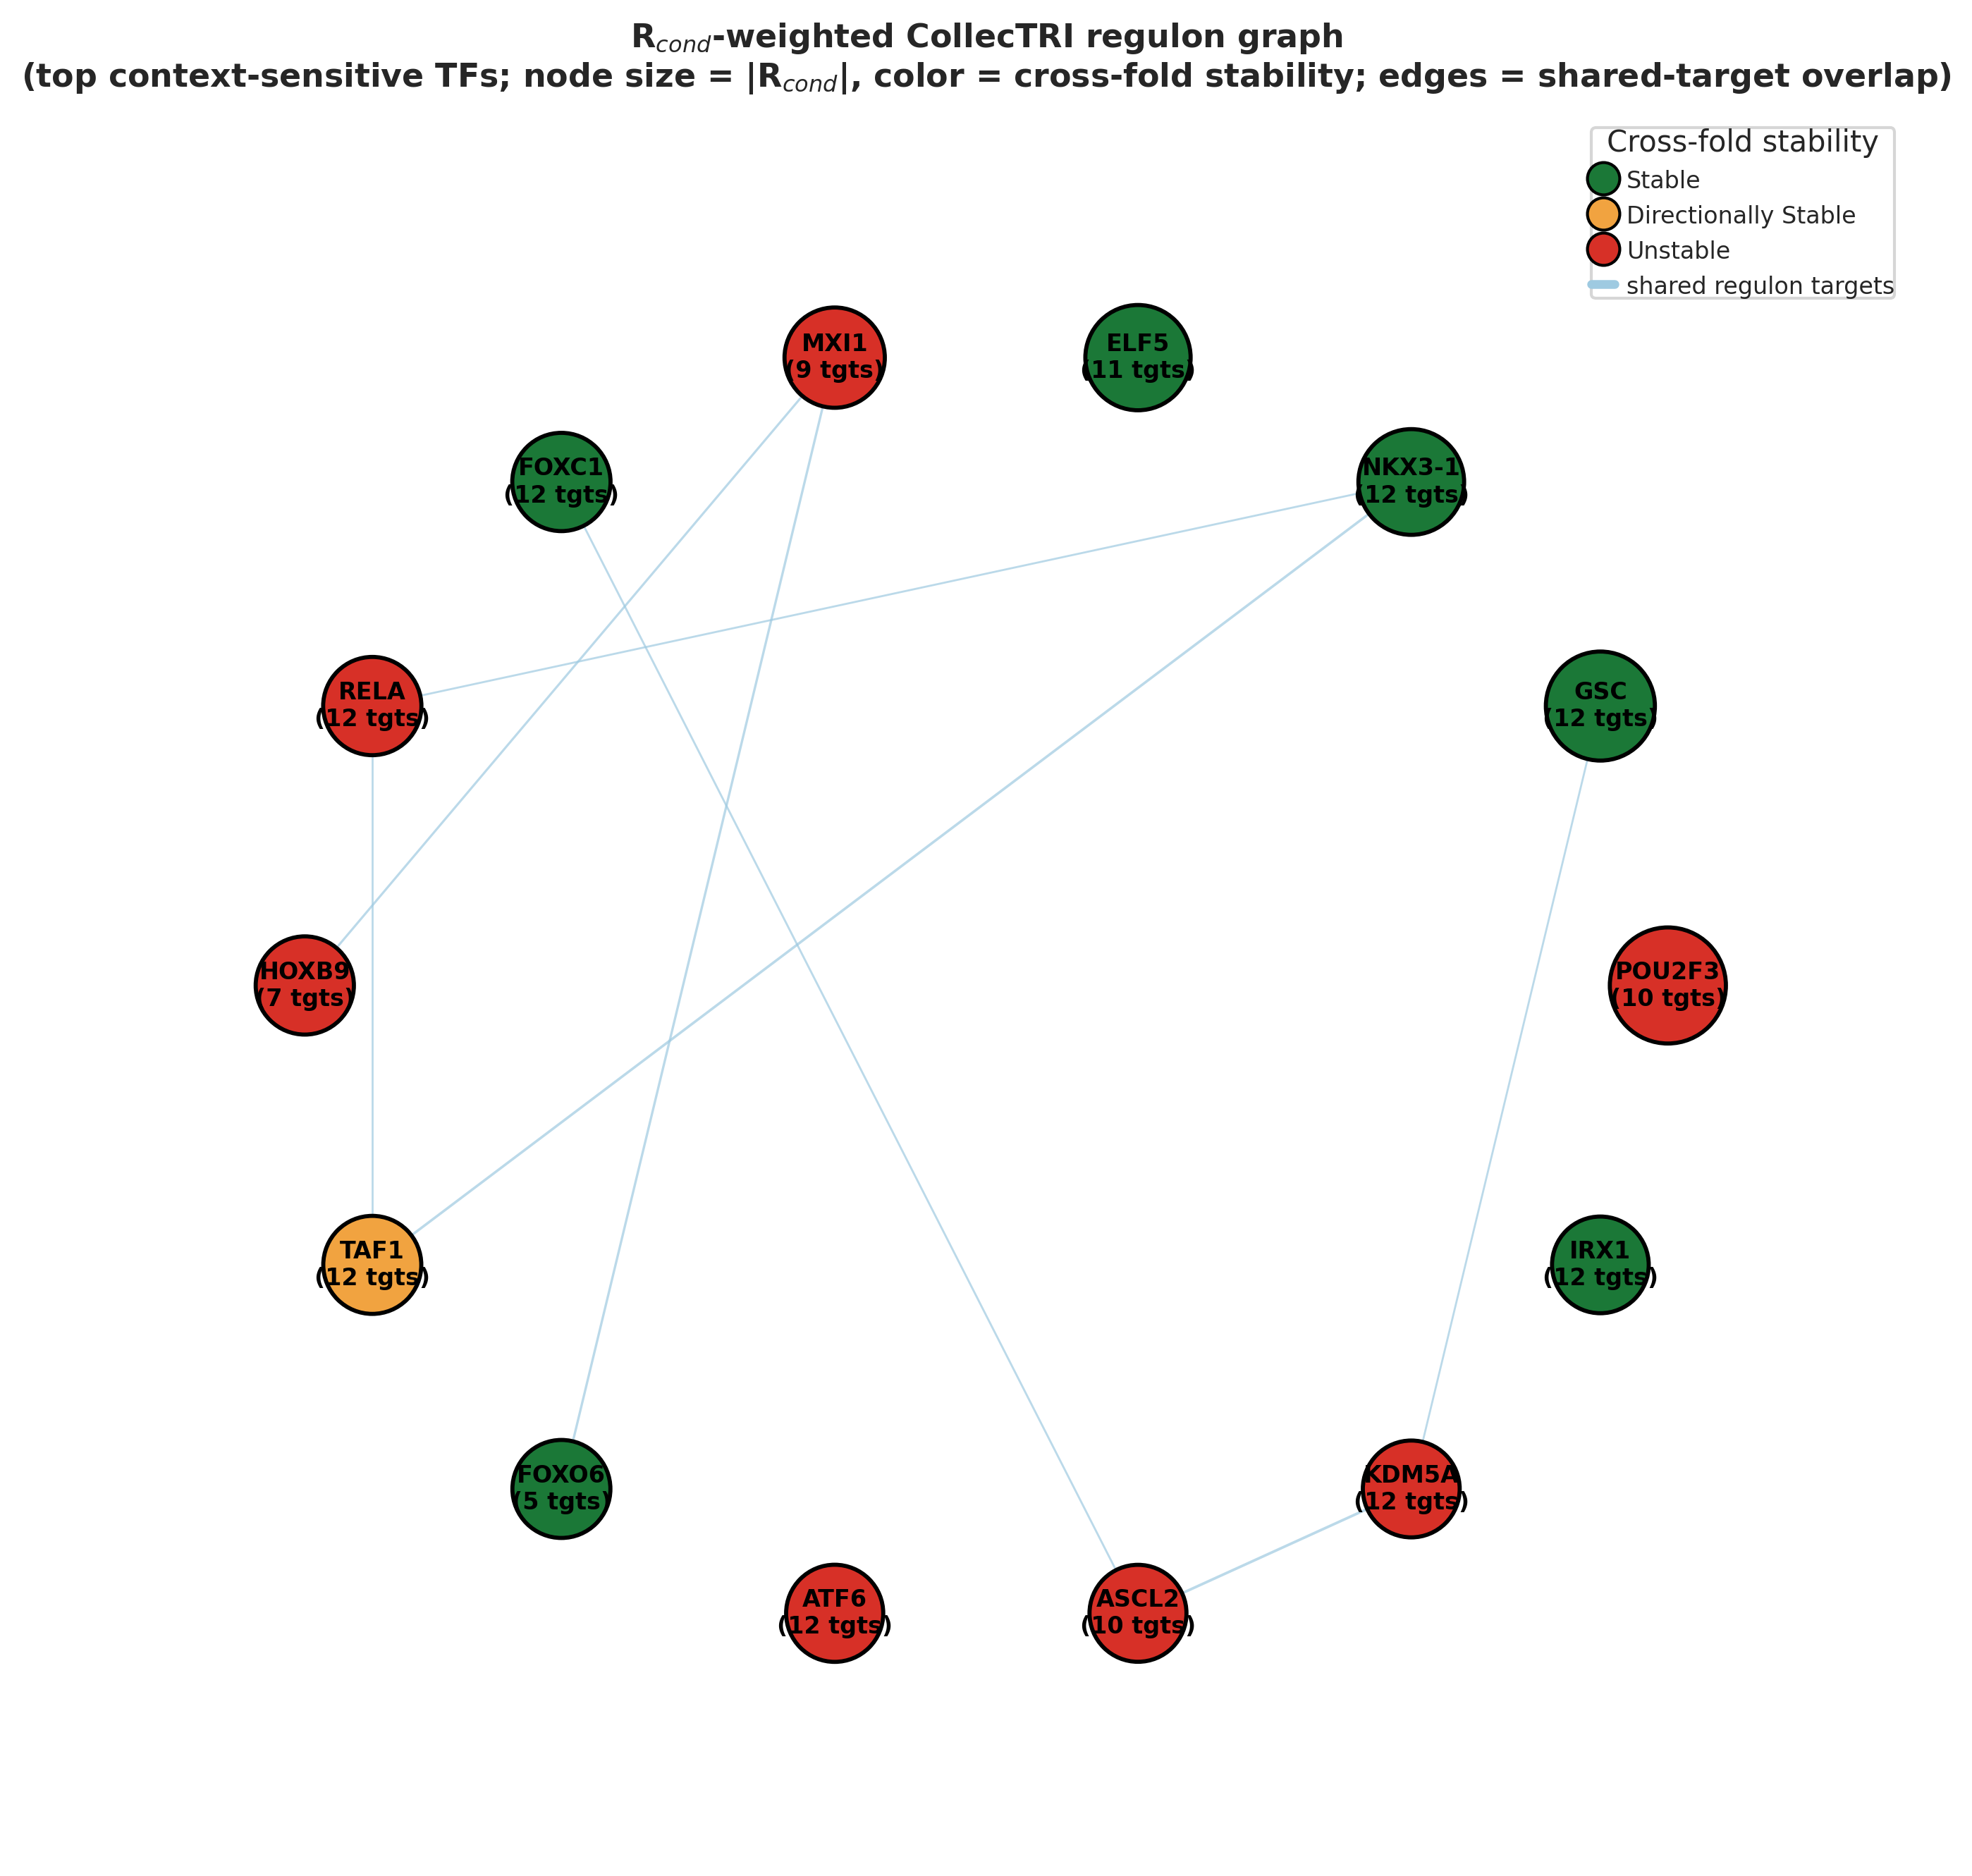
\includegraphics[width=0.9\textwidth]{figures/fig_rcond_regulon_network.png}
  \caption[Context-annotated regulon network, AAH$\rightarrow$AIS]{Force-directed CollecTRI regulon network for the stable and directionally-stable transcription factors on the AAH$\rightarrow$AIS edge. Node fill encodes the signed context effect $R_{\text{cond}}$ (diverging scale: red context-upregulated, blue context-downregulated) and node border encodes cross-fold stability. The layout situates the context-upregulated AP-1 factor FOS and the context-downregulated interferon regulator IRF9 within their regulatory neighborhoods.}
  \label{fig:regulon_network}
\end{figure}

\section{At the invasion boundary, transport sustains WNT while suppressing VEGF}
\label{sec:invasion-signature}

The same estimand was applied to the AIS$\rightarrow$invasive edge, pooling minimally invasive and invasive LUAD as the target stage. Twenty-eight programs are STABLE and 38 are DIRECTIONALLY\_STABLE of 773. Among pathways, WNT and TRAIL remain stably context-upregulated (WNT $+0.287$; 95\% CI, $+0.227$ to $+0.339$; TRAIL $+0.281$; $+0.251$ to $+0.311$), and VEGF is the largest-magnitude stable pathway, redirected downward ($-0.318$; $-0.374$ to $-0.229$). The stable transcription factors include the Notch coactivator MAML1 ($+0.292$; $+0.258$ to $+0.325$), the endoderm/lineage factor FOXA1 ($+0.192$), the stress factor ATF5 ($+0.182$), and NFKB2 ($+0.145$), against context-downregulated CTBP1 ($-0.202$) and NAB2 ($-0.176$). WNT-pathway upregulation is thus sustained across both the preinvasive and the invasion edge, while VEGF suppression is specific to the invasion boundary.

\section{A metabolic and interferon program reverses direction between the preinvasive and invasive transitions}
\label{sec:gsea}

The regulatory-transport estimand isolates the context-conditioned component of progression; as an
orthogonal, model-independent description of the same edges, stage differential expression was ranked
by gene-set enrichment (fgsea over GO Biological Process and MSigDB Hallmark collections; positive
normalized enrichment score, NES, denotes upregulation at the target stage). The two edges are not
simply stronger and weaker versions of one transition---they carry opposite metabolic and immune
signatures.

At the preinvasive AAH$\rightarrow$AIS transition, the upregulated programs are dominated by ciliary and
mucosal-immune biology (axoneme assembly, NES $+2.16$; cilium movement, $+2.15$; mucosal immune
response, $+2.03$; all $q<0.001$), while oxidative metabolism and interferon signaling are
coordinately \emph{downregulated} (\textsc{hallmark\_oxidative\_phosphorylation}, NES $-1.84$;
\textsc{hallmark\_interferon\_gamma\_response}, $-1.85$; \textsc{hallmark\_interferon\_alpha\_response},
$-1.75$; \textsc{hallmark\_myc\_targets\_v1}, $-1.68$; all $q<0.001$; Fig.~\ref{fig:gsea_aah_ais}).
At the AIS$\rightarrow$invasive transition the same four programs \emph{reverse sign}: oxidative
phosphorylation ($+1.81$), interferon-$\gamma$ ($+1.78$) and interferon-$\alpha$ ($+1.80$) responses,
and MYC targets ($+1.92$) are now all upregulated, while sensory-perception and ciliary programs
collapse (sensory perception of chemical stimulus, NES $-2.61$, the strongest single enrichment on
either edge; cilium movement, $-1.97$; $q<0.001$; Fig.~\ref{fig:gsea_ais_inv}). The coordinated
reversal of the oxidative-phosphorylation, interferon, and MYC axes distinguishes the two transitions:
the preinvasive step suppresses oxidative metabolism and interferon tone while retaining a ciliated
epithelial identity, whereas the invasive step restores oxidative metabolism and interferon signaling
and engages MYC-driven proliferation as ciliary identity is lost. This whole-transcriptome
description is concordant with the context-residual reading---JAK-STAT (interferon-effector) redirection
is downregulated at the preinvasive edge under $R_{\text{cond}}$ (Section~\ref{sec:stable})---and
provides the biological backdrop against which the niche-conditioned transport effects are interpreted.

\begin{figure}[htbp]
  \centering
  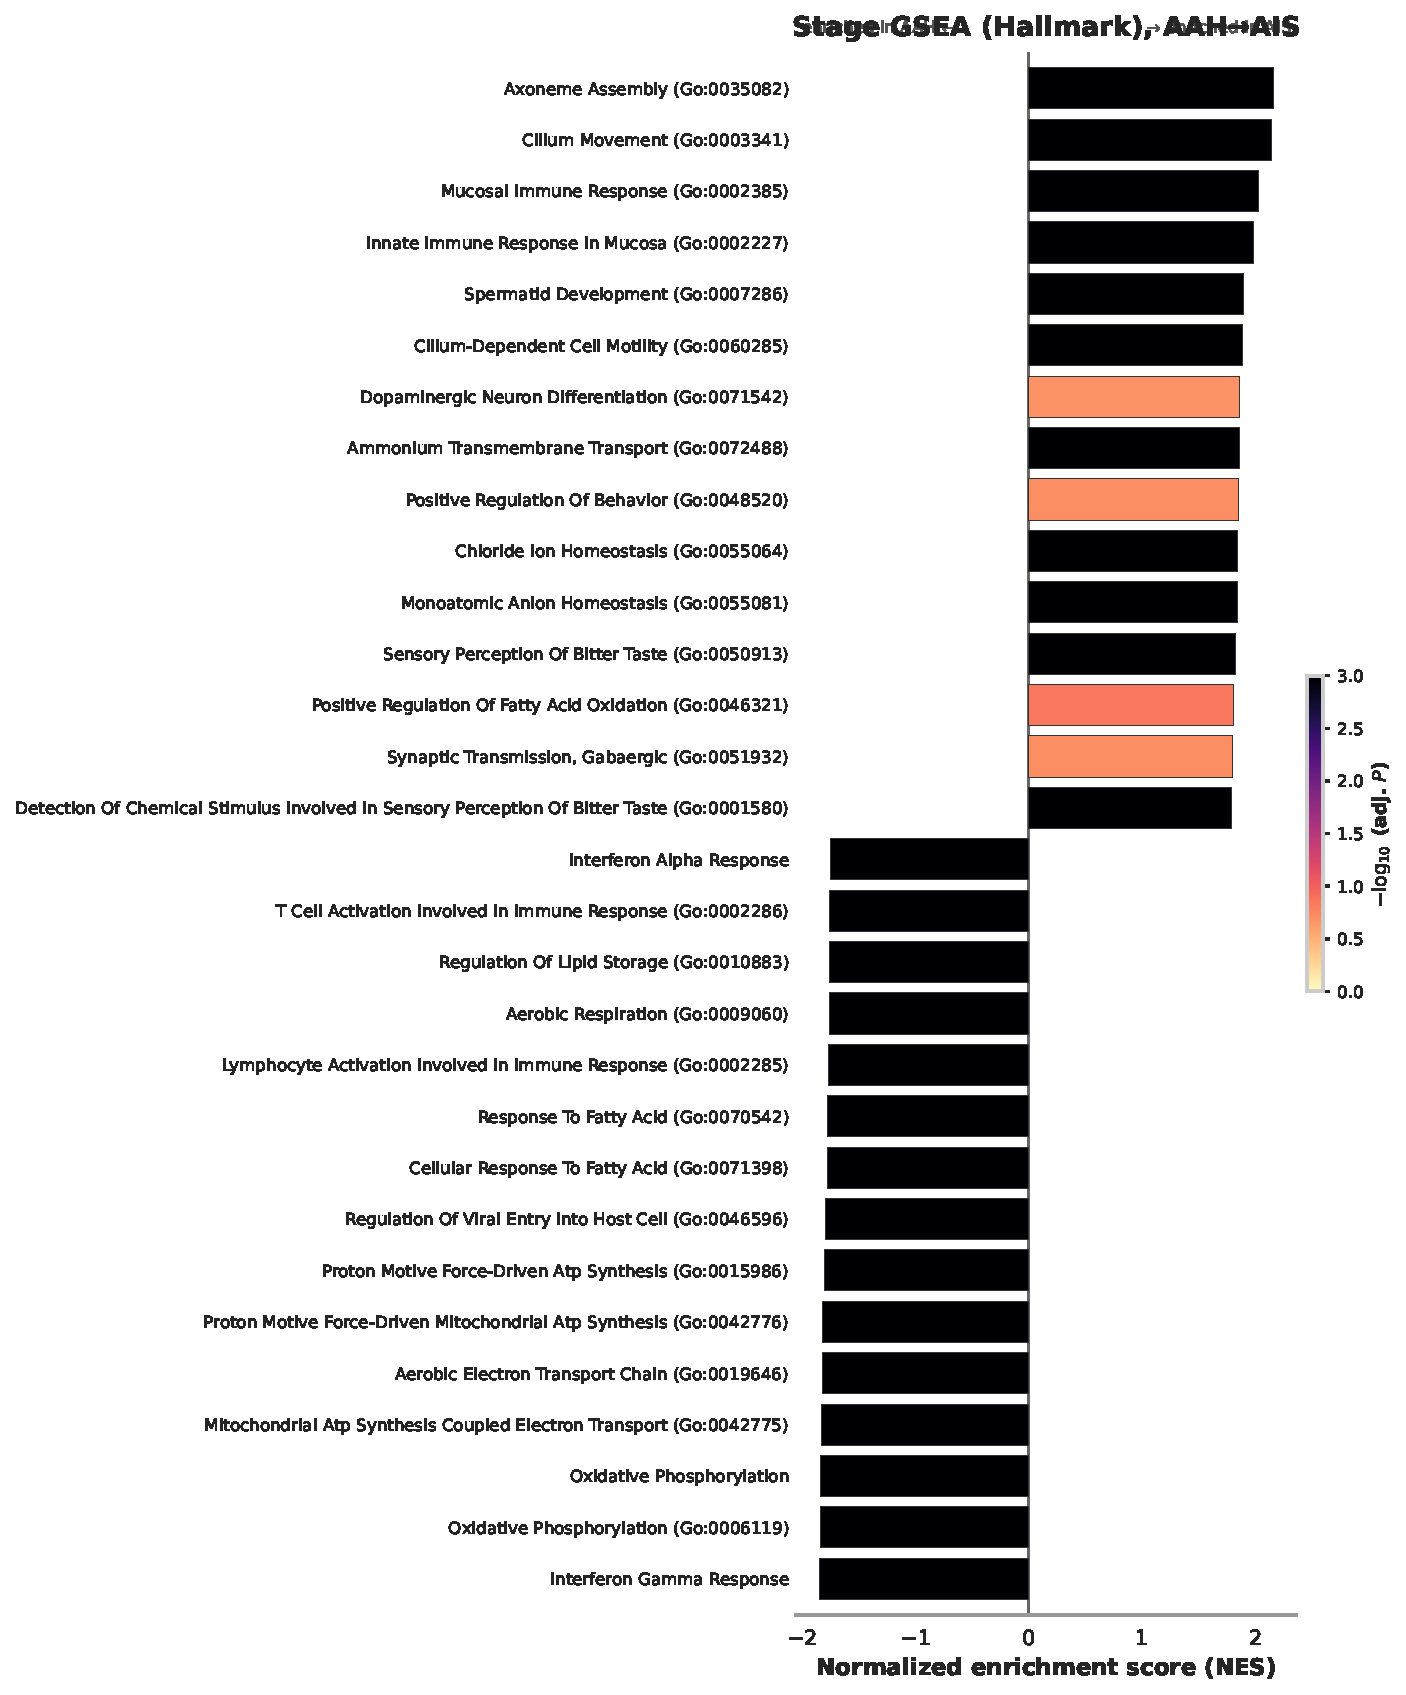
\includegraphics[width=0.9\textwidth]{figures/gsea/stage_gsea_bar_AAH_AIS.pdf}
  \caption[Stage gene-set enrichment, AAH$\rightarrow$AIS]{Signed gene-set enrichment for the
  AAH$\rightarrow$AIS transition (fgsea; bar = normalized enrichment score, positive = upregulated at
  AIS). Ciliary and mucosal-immune programs are upregulated; oxidative phosphorylation, interferon-$\gamma$/$\alpha$,
  and MYC targets are coordinately downregulated. Of $93$ significant gene sets ($q<0.05$), $27$ are
  up and $66$ down.}
  \label{fig:gsea_aah_ais}
\end{figure}

\begin{figure}[htbp]
  \centering
  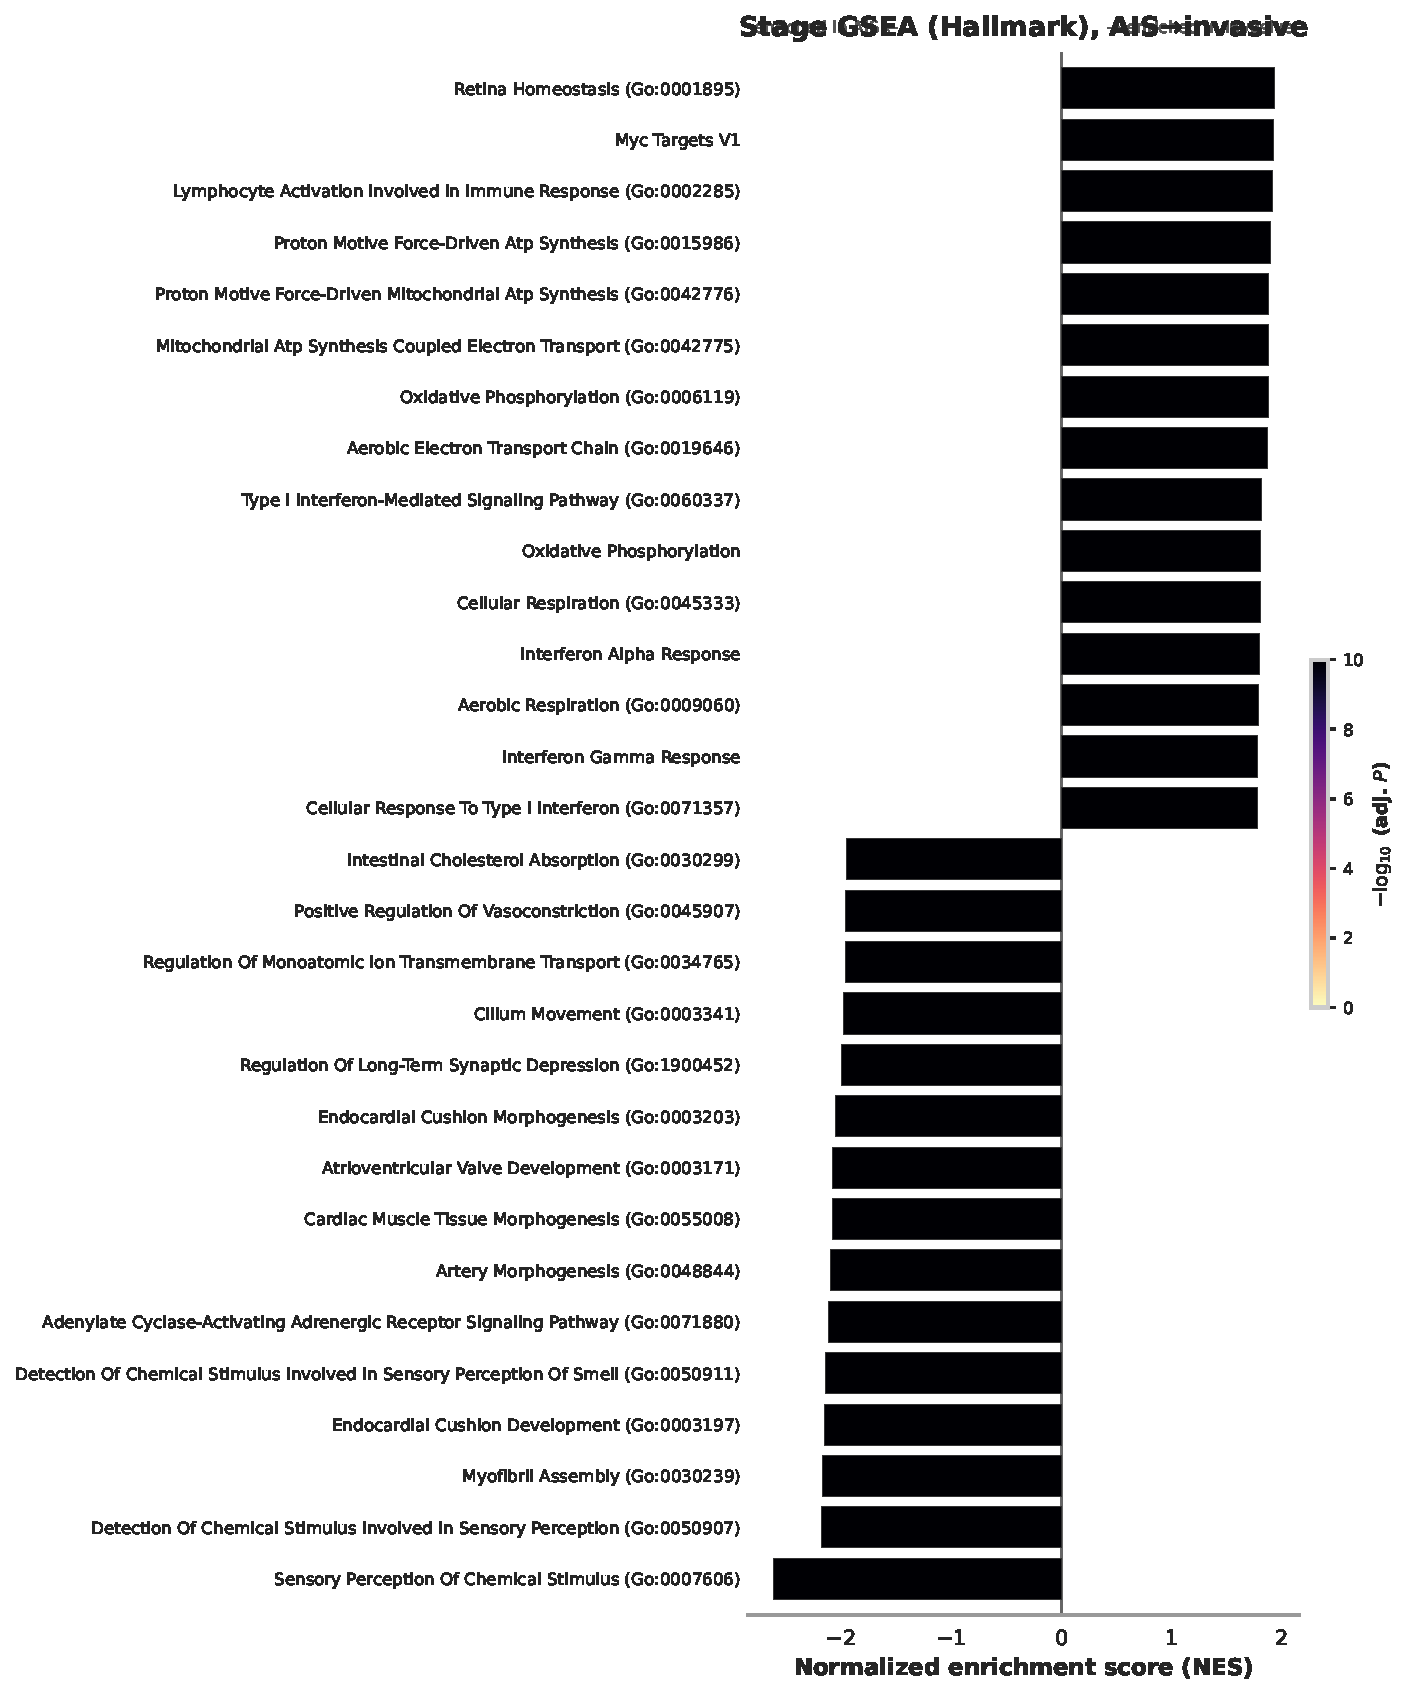
\includegraphics[width=0.9\textwidth]{figures/gsea/stage_gsea_bar_AIS_invasive.pdf}
  \caption[Stage gene-set enrichment, AIS$\rightarrow$invasive]{Signed gene-set enrichment for the
  AIS$\rightarrow$invasive transition. Oxidative phosphorylation, interferon-$\gamma$/$\alpha$, and MYC
  targets---all downregulated at the preinvasive edge---are now upregulated, while sensory-perception
  and ciliary programs are strongly downregulated (sensory perception of chemical stimulus, NES
  $-2.61$). Of $180$ significant gene sets, $122$ are up and $58$ down.}
  \label{fig:gsea_ais_inv}
\end{figure}

\section{Co-expression network modules are directionally concordant with the regulatory-transport signature}
\label{sec:grn}

To assess whether the niche-redirected programs identified by regulatory transport are recovered by independent analytic methods on the same data, we applied pySCENIC de-novo regulon inference and hdWGCNA weighted co-expression network analysis to the same epithelial atlas. These analyses operate on raw co-expression structure with no knowledge of the CRRT-UDE estimand, but because they read the same expression matrix, their agreement with the R\textsubscript{cond} signature is cross-method consistency rather than an independent measurement modality, and is interpreted with that limit in mind.

\paragraph{pySCENIC regulons.} GRNBoost2 co-expression inference followed by cisTarget motif pruning identified 3,993 motif-supported regulons on the AAH$\rightarrow$AIS edge and 4,675 on AIS$\rightarrow$invasive, spanning 1.75 and 1.83 million co-expression edges respectively. Several stable or directionally-stable R\textsubscript{cond} transcription factors also appear among the SCENIC regulators, including FOS, RB1, IRF9, ETV3, ETV6, SMAD4, FOXA1, and NFKB2. This overlap is descriptive rather than a statistical corroboration: the adjacency graph contains $1{,}753$ regulators spanning nearly all scored transcription factors, so appearance in the graph is close to automatic, and a hypergeometric test against the highest-out-degree regulators finds the stable-TF overlap no greater than chance ($0.95$--$1.14\times$; $P = 0.35$--$0.63$). The named factors are therefore reported as regulators that are both context-driven under R\textsubscript{cond} and present in the de-novo network, not as an enriched intersection. The relationship between regulon stage-specificity and context effect, and the per-cell regulon-activity structure, are shown in Appendix~\ref{sec:app-c-grn} (Figures~\ref{fig:rss_vs_rcond} and \ref{fig:scenic_clustermap}).


\paragraph{hdWGCNA modules and GO enrichment.} Weighted co-expression clustering identified seven reproducible modules per edge (SM1--SM7, plus unassigned grey). Module identity is stable across the two LUAD edges: SM1 ($n=67$--$82$ genes; hub genes MS4A2, HDC, CPA3, TPSD1) is a mast-cell module; SM2 ($n=356$--$411$; hub genes ITGAL, ZAP70, TRAC, CD2) is a T-cell module; SM3 ($n=89$--$91$; hub genes NKX2-1, SFTA3, AQP4) is an alveolar epithelial identity module; SM4 ($n=309$--$327$; hub genes EGFL7, CDH5, VWF, CALCRL) is a vascular/endothelial module; SM5 shifts between edges (AAH$\rightarrow$AIS: ciliated epithelial; AIS$\rightarrow$invasive: macrophage/monocyte, hub genes MS4A7, CD163, CSF1R, C1QB); SM6 ($n=114$--$444$) is a stromal/ECM module (COL6A1, COL1A2, ELN); and SM7 is a cilia/dynein module. The module architecture and its GO enrichment are shown in Appendix~\ref{sec:app-c-grn} (Figures~\ref{fig:module_umap} and \ref{fig:module_enrichment}).

Gene-set enrichment (fgsea, GO Biological Process) identified the vascular SM4 module as enriched for regulation of cell migration (padj $= 0.007$, NES $= 1.95$), TGF$\beta$ response (padj $= 0.061$, NES $= 1.86$), MAPK cascade (padj $= 0.061$), and angiogenesis regulation (padj $= 0.089$) on the AAH$\rightarrow$AIS edge. At invasion, the macrophage SM5 module is the only module with a significantly negative NES: it is enriched for chemokine-mediated signaling (padj $= 0.019$, NES $= -2.07$) and cellular response to chemokine (padj $= 0.019$, NES $= -2.07$), indicating that chemokine-high macrophage co-expression is down-weighted at the invasion boundary. The stromal SM6 module gains significance at invasion with supramolecular fiber organization (padj $= 0.052$, NES $= 1.82$; leading-edge genes COL1A1, COL3A1, LTBP2, COL5A2), consistent with an ECM-remodeling signal specific to the invasive transition.

These module-level findings are directionally concordant with the R\textsubscript{cond} signature in three respects. First, VEGF suppression and TGF$\beta$ downregulation in R\textsubscript{cond} at invasion are mirrored by the vascular SM4 module's stable enrichment for TGF$\beta$ response and growth factor signaling at both edges, while the chemokine-negative SM5 signal at invasion is consistent with the JAK-STAT downregulation ($-0.246$) observed in R\textsubscript{cond} at the preinvasive step. Second, the R\textsubscript{cond} upregulation of FOS (AP-1) and the SCENIC adjacency evidence for FOS as a major regulatory hub are mutually reinforcing: FOS is nominated by both co-expression topology and the model-based context test. Third, the stromal SM6 ECM module, which gains significance only at invasion, is consistent with the VEGF-suppressed, Notch/FOXA1-upregulated R\textsubscript{cond} invasion signature, both pointing to a stromal remodeling event that distinguishes the invasive from the preinvasive transition.

\section{An $R_{\text{cond}}$-gated framework links intercellular signaling to context-driven regulatory programs}
\label{sec:comm}

The context-residual estimand supports a mechanistic extension that nominates the intercellular signals plausibly responsible for each context-driven regulatory program. Ligand-receptor interactions are inferred by LIANA consensus across cell types at each stage, receptor$\rightarrow$transcription-factor wiring is drawn from OmniPath post-translational interactions, and each sender$\rightarrow$ligand$\rightarrow$receptor$\rightarrow$TF chain is retained only when its terminal TF program is classified \textsc{stable} or \textsc{directionally\_stable} with $|R_{\text{cond}}| \geq 0.05$ on that edge. This model-based gate is what distinguishes the framework from co-expression-based cell--cell communication tools: rather than ranking interactions by expression correlation alone, it retains only those channels whose downstream regulatory program the dynamical model independently identifies as context-driven. Downstream target genes of each gated TF are drawn from CollecTRI, and Ollivier--Ricci curvature of the differential communication network is used to nominate structural bottleneck channels that reorganize across the stage edge.

Applied to the full LUAD cohort, the gate is highly selective. On the AAH$\rightarrow$AIS edge ($209{,}879$ epithelial and stromal cells, $77$ cell types), LIANA nominated $583{,}547$ ligand--receptor interactions at AAH and $657{,}529$ at AIS, expanding to roughly $1.1$ and $1.3$ million candidate sender$\rightarrow$ligand$\rightarrow$receptor$\rightarrow$TF chains; after $R_{\text{cond}}$-gating, the top-ranked retained chains resolve onto just two programs, both already established as stable in Section~\ref{sec:stable}: the AP-1 factor FOS ($R_{\text{cond}}$ $+0.141$) and RB1 ($+0.110$). The surviving chains are dominated by macrophage- and stromal-derived signaling into these programs---APOE, GRN, PSAP, and A2M from alveolar and CHIT1$^{+}$ macrophages, and LTF, C3, and PLA2G2A from mesothelial and serous-gland cells, routed through the LRP1 and EGFR receptors (Figure~\ref{fig:comm_chain}). The EGFR$\rightarrow$FOS chains give an intercellular reading of the AP-1 upregulation reported at this edge, and the LRP1$\rightarrow$RB1 chains implicate scavenging-receptor signaling from the myeloid and stromal compartment. On the AIS$\rightarrow$invasive edge ($553{,}298$ cells), the gated chains resolve onto a larger stable set---CTBP1 ($-0.202$), FOXA1 ($+0.192$), and STAT5B ($+0.140$), together with the directionally-stable HDAC1 ($-0.204$) and HSF2 ($+0.225$)---with fibroblast- and macrophage-derived DCN, GRN, and PSAP again routed predominantly through EGFR.

These chains are mechanistic \emph{nominations}, not validated interactions, and they are consistent with---not in tension with---the bounded endpoint result of Section~\ref{sec:results-ladder}. The gate operates at the level of \emph{which programs are reproducibly context-driven}, a claim the per-program analysis supports, and not at the level of endpoint prediction, where local niche did not separate from shuffled context. The framework therefore proposes the intercellular signals plausibly feeding the reproducible program residuals, generating specific, testable sender--ligand--receptor hypotheses (macrophage APOE/GRN$\rightarrow$LRP1/EGFR$\rightarrow$FOS/RB1 in the preinvasive niche) for targeted follow-up. As with the co-expression analysis, the ligand--receptor inference and the gate read the same expression matrix, so the chains are hypotheses generated internally to the data rather than an independent confirmation.

Beyond the gated chains, the communication \emph{network} itself reorganizes across the preinvasive edge. Ollivier--Ricci curvature---a measure for which negative values mark edges through which signaling mass is funneled, i.e.\ structural bottlenecks---was computed on the differential ligand--receptor network, and $1{,}588$ of its $2{,}415$ channels ($66\%$) become more bottlenecked at AIS (mean $\Delta\kappa = +0.089$; Figure~\ref{fig:ricci_diff}). The strongest emerging bottlenecks route through submucosal-gland and innate-lymphoid senders (SMG-mucous$\rightarrow$$\gamma\delta$T, $\Delta\kappa = -0.49$; ILC$\rightarrow$secretory and neuroendocrine channels), identifying the submucosal-gland/ILC hub as the locus of greatest network reorganization at the preinvasive transition; the full curvature tables and the invasion-edge network are given in Appendix~\ref{sec:app-c-comm}.

\begin{figure}[htbp]
  \centering
  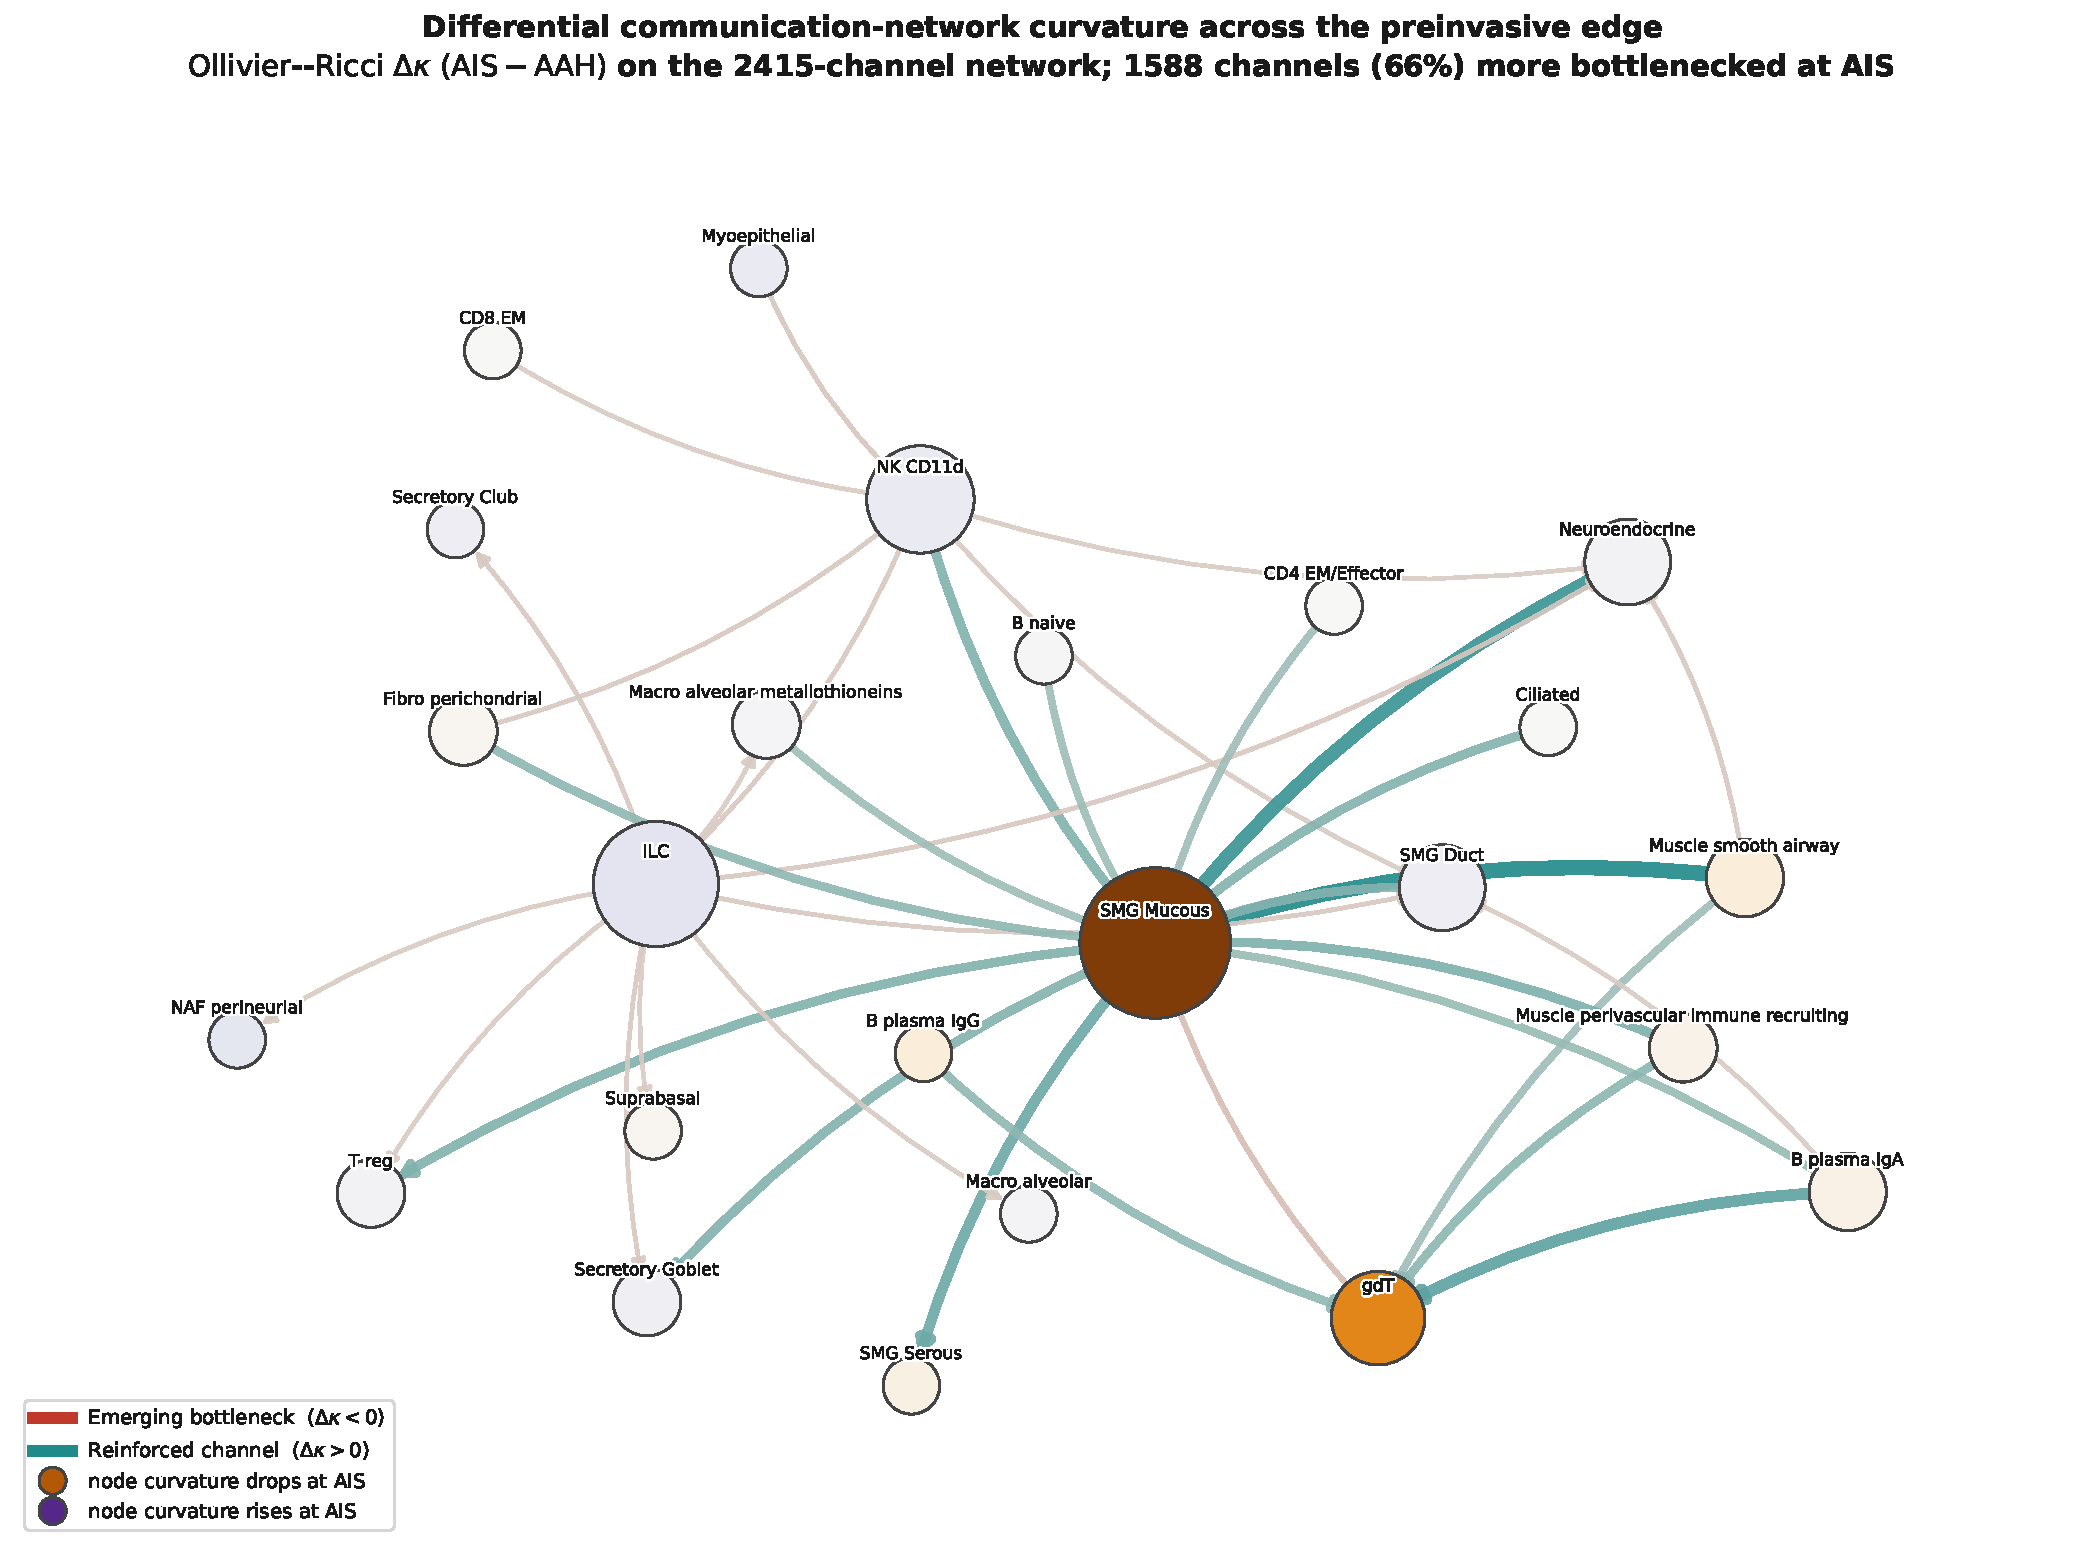
\includegraphics[width=0.95\textwidth]{figures/comm/ricci_differential_curvature_AAH_AIS.pdf}
  \caption[Differential communication-network curvature, AAH$\rightarrow$AIS]{Ollivier--Ricci
  differential curvature $\Delta\kappa$ (AIS $-$ AAH) on the cell--cell communication network. Nodes are
  cell types (sized by involvement in the most-reorganized channels, colored by node-level curvature
  change); edges are the most-reorganized channels, colored from emerging bottleneck
  ($\Delta\kappa<0$) to reinforced ($\Delta\kappa>0$). The submucosal-gland-mucous node is the central
  hub of reorganization, with signaling into $\gamma\delta$T and secretory populations funneling
  (curvature dropping) at AIS. This is a descriptive network summary of the LIANA differential network,
  not an $R_{\text{cond}}$-gated quantity.}
  \label{fig:ricci_diff}
\end{figure}

\begin{figure}[htbp]
  \centering
  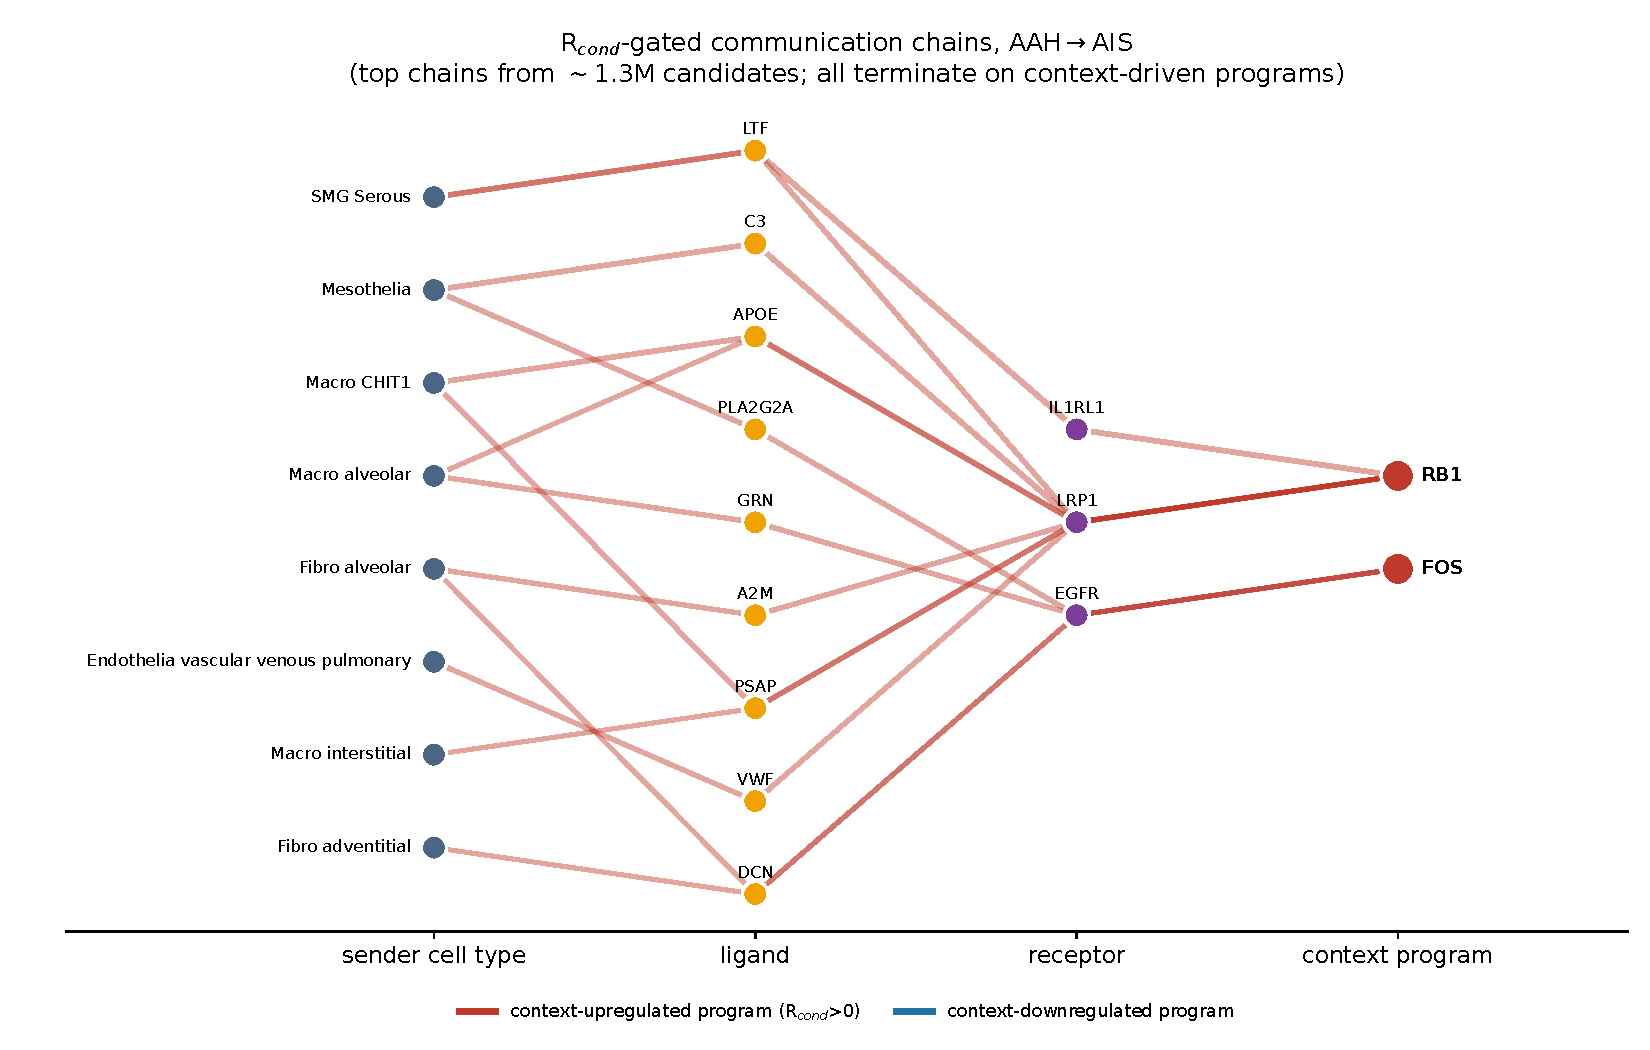
\includegraphics[width=0.95\textwidth]{figures/comm/gated_chain_AAH_AIS.pdf}
  \caption[$R_{\text{cond}}$-gated communication chains, AAH$\rightarrow$AIS]{Top $R_{\text{cond}}$-gated
  sender$\rightarrow$ligand$\rightarrow$receptor$\rightarrow$context-program chains retained on the
  AAH$\rightarrow$AIS edge, from roughly $1.3$ million candidates. Only chains terminating on a
  context-driven program (stable or directionally-stable $R_{\text{cond}}$) survive the gate; the
  retained chains route macrophage- and stromal-derived ligands (APOE, GRN, PSAP, A2M, LTF, C3) through
  the LRP1 and EGFR receptors onto the FOS and RB1 programs. Edge width is the gated chain score and
  edge color is the sign of the terminal program's context effect. The chains are mechanistic
  nominations for the intercellular signals feeding the reproducible program residuals, not validated
  interactions.}
  \label{fig:comm_chain}
\end{figure}

\section{The estimand transfers to pancreatic precursors without over-calling stability}
\label{sec:panin}

The same estimand was applied to a graded PanIN series (low-grade $\rightarrow$ high-grade) as a cross-disease transferability and null-calibration probe. This series is underpowered by design: it comprises roughly four donors and on the order of one hundred graded receivers. The powered stability filter returns zero STABLE programs; 188 programs are DIRECTIONALLY\_STABLE under a confidence-interval-excludes-zero filter, and the remainder are unstable. Zero stable programs at four donors is the expected behavior of a patient-resampling filter that cannot manufacture cross-patient stability from a cohort this small; it is reported as the estimator declining to over-call rather than as a positive demonstration of calibration, because with no positive control at matched sample size a true null and simple lack of power are not separable here. This limit is stated plainly and PanIN is not used to license any LUAD claim.

Despite being underpowered, the directionally consistent programs are biologically coherent. Inflammatory and growth pathways separate in direction, with NF$\kappa$B context-upregulated ($+0.382$, directionally stable) and EGFR context-upregulated ($+0.291$, unstable at this cohort size), consistent with an inflammatory-to-proliferative shift during PanIN progression \autocite{Bell2024-kn} (Fig.~\ref{fig:panin-forest}). PanIN is therefore reported as a transferability probe, not as calibration evidence.

\begin{figure}[htbp]
  \centering
  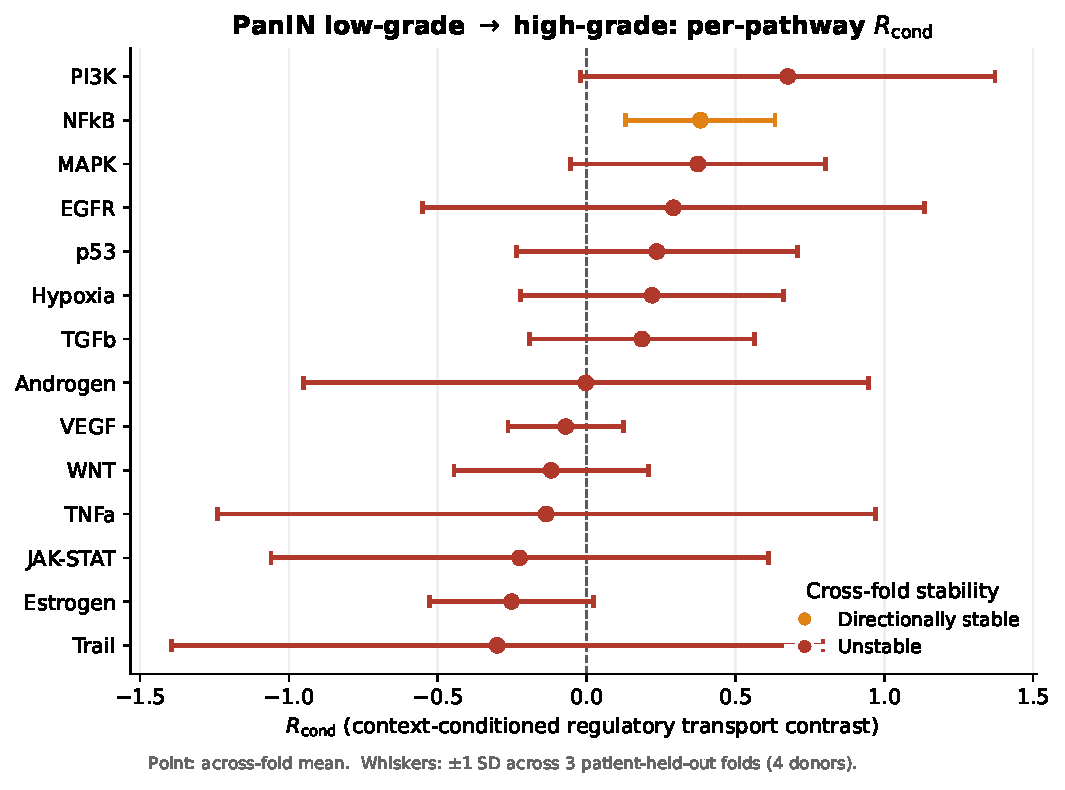
\includegraphics[width=0.82\textwidth]{figures/appendix/panin_pathway_forest.pdf}
  \caption[Cross-disease PanIN pathway transport]{Per-pathway conditional transport $R_{\text{cond}}$ on
  the cross-disease PanIN low-grade$\rightarrow$high-grade edge (14 PROGENy pathways). Points are
  across-fold means; whiskers span $\pm1$ SD over the three patient-held-out folds (4 donors). Only
  NF$\kappa$B is directionally stable (interval off zero, sign-consistent, orange); every other pathway
  is unstable with a wide interval straddling zero---the expected underpowered null at this cohort size.
  The one coherent signal, context-upregulated NF$\kappa$B beside directionally-upregulated EGFR, matches
  an inflammatory-to-proliferative shift. PanIN is a transferability probe, not calibration evidence.}
  \label{fig:panin-forest}
\end{figure}

The inflammatory signal has a spatial correlate. Immune abundance in these sections is not diffuse but organized into discrete foci: a Getis--Ord Gi* hot-spot analysis of the per-spot immune fraction resolves compact, statistically significant immune-enriched neighbourhoods within every PanIN section (Fig.~\ref{fig:panin-getis}), the same focal microenvironmental structure seen on the LUAD edge (Fig.~\ref{fig:spatial_autocorr_maps}). The context-upregulated NF$\kappa$B signal therefore sits in a tissue whose immune compartment is spatially structured rather than well-mixed, which is the local ecology such a niche-gated term would draw on.

\begin{figure}[htbp]
  \centering
  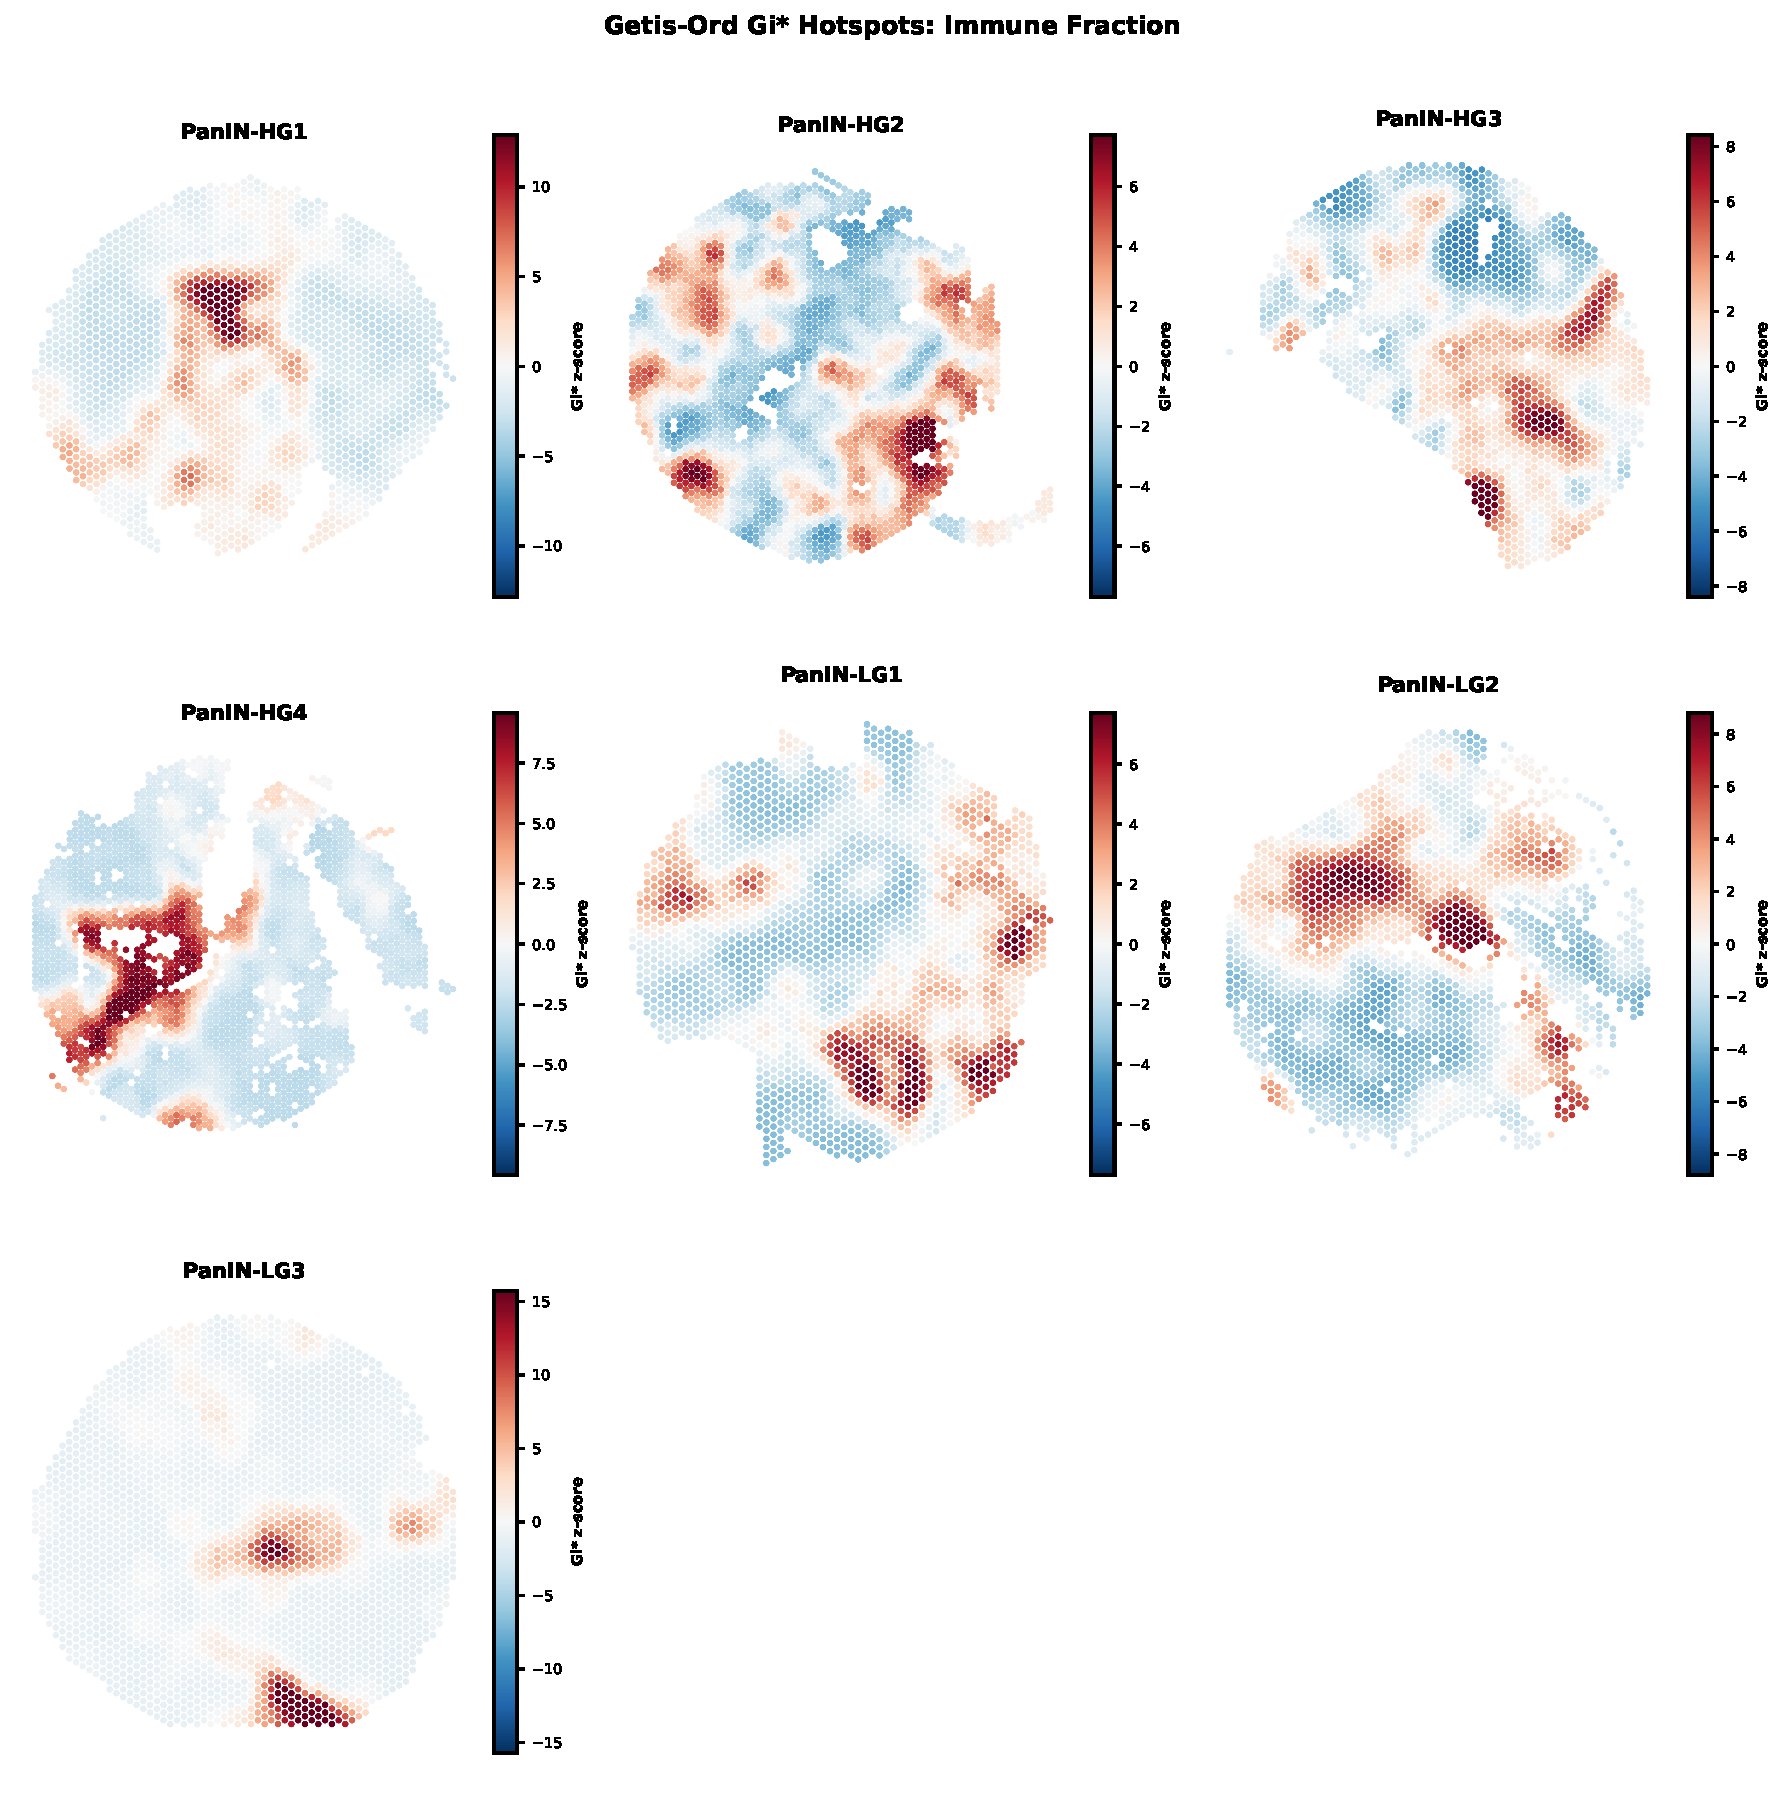
\includegraphics[width=\textwidth]{figures/spatial/panin_getis_immune.pdf}
  \caption[Immune hot spots in the PanIN sections]{Getis--Ord Gi* hot-spot $z$-scores for the per-spot
  immune fraction in each PanIN section (tissue coordinates; red = immune-enriched neighbourhood,
  blue = immune-depleted). Every section resolves compact, spatially contiguous immune-enriched foci
  rather than a uniform immune background---the focal microenvironmental structure a niche-gated term
  draws on, and the cross-disease counterpart of the LUAD spatial organization (Fig.~\ref{fig:spatial_autocorr_maps}).
  Descriptive per-section rendering, not a statistical test of progression.}
  \label{fig:panin-getis}
\end{figure}

\section{Local niche context is equivalent to shuffled context and only suggestively better than self-only}
\label{sec:results-ladder}

The falsification ladder tests whether local niche context improves prediction of the AIS endpoint over coarser specimen-level and self-only alternatives, scored by semantic Sinkhorn distance (lower is better, mean over five folds; Table~\ref{tab:ladder}). Local niche transport (local\_context\_full, $123.65$) has a lower mean distance than spatial self-only transport ($132.41$) and is favored in four of five patient-held-out folds, but the paired difference is underpowered: $+8.76$ (paired $95\%$ CI $[-2.83, +20.35]$, $P \approx 0.10$), so the interval includes zero and the self-only advantage is directionally consistent rather than established. The degenerate single-branch fields, by contrast, collapse unambiguously: a structured-only field reaches $2621.22$ and a residual-only field $654.81$, so neither half of the grey-box decomposition reproduces the transport alone.

That is the extent of the claim; the table bounds it in three further ways. First, local context does not separate from a specimen-level average (donor\_stage\_average\_context, $122.97$) or, decisively, from its own stratum-matched shuffle (matched\_state\_shuffled, $123.73$). The shuffle contrast is an \emph{equivalence bound} rather than a bare failure to reject: on the five shared patient-held-out folds, the paired local-over-shuffle difference is $+0.08$ (paired $95\%$ CI $[-1.10, +1.26]$, $P = 0.86$), so any local-context endpoint benefit above about $1.3$ Sinkhorn units is excluded, and cell-resolved niche and permuted niche predict the endpoint equally well. The two contrasts carry very different precision, and the reason is structural: the stratum-matched shuffle preserves the marginal structure of the context, so its transport co-moves with the local model fold-for-fold and the paired difference is tight (standard deviation of the fold-level difference $\approx 1.0$), whereas the self-only model is a structurally different field, so its fold-level differences swing widely (standard deviation $\approx 9.3$) and the same five folds cannot resolve the $+8.76$ mean gap from zero. The well-powered claim is therefore the equivalence to shuffled context; the self-only advantage is suggestive but underpowered. Second, an unstructured neural field (monolithic\_nn, $121.59$) fits better than the structured decomposition---the expected cost of trading raw fit for an interpretable, program-resolved field. Third, the strict-$z$ coupling rejected during estimand selection attains the best fit in the table (strict\_z\_full, $119.17$; and even strict\_z\_self\_only, $123.13$, edges out the local model). This is expected and not a reversal of the selection: the endpoint metric is a Sinkhorn distance scored in the same regulatory $z$-space that strict-$z$ coupling is constructed to optimize, so the metric is near-circular in strict-$z$'s favor. The coupling was selected on Tier-2 regulatory recovery in the prespecified synthetic benchmark (Section~\ref{sec:results-estimand}), not on endpoint fit, because endpoint fit in $z$-space cannot arbitrate between couplings without this circularity. The honest reading of the ladder is therefore bounded and split by contrast: local context is directionally but not significantly better than self-only ($P \approx 0.10$), is equivalent to shuffled context within a tight bound, does not beat specimen-level ecology, and does not win the endpoint metric outright.

\begin{table}[htbp]
  \centering
  \caption[AAH$\rightarrow$AIS falsification ladder]{AAH$\rightarrow$AIS falsification ladder, mean semantic Sinkhorn distance over five folds (lower is better). local\_context\_full has a lower mean than spatial\_self\_only and is favored in 4/5 folds, but the paired difference is underpowered ($+8.76$, $95\%$ CI $[-2.83, +20.35]$, $P \approx 0.10$); the structured-only and residual-only degenerate fields collapse unambiguously, supporting the grey-box decomposition. Local context is statistically equivalent to its stratum-matched shuffle (paired $+0.08$, $[-1.10,+1.26]$), so the well-powered claim is equivalence at the receiver-local scale, not a local advantage over self-only or specimen-level ecology.}
  \label{tab:ladder}
  \begin{tabular}{lc}
    \toprule
    Ladder rung & Sinkhorn distance \\
    \midrule
    strict\_z\_full               & 119.17 \\
    monolithic\_nn                & 121.59 \\
    donor\_stage\_average\_context & 122.97 \\
    strict\_z\_self\_only          & 123.13 \\
    local\_context\_full          & 123.65 \\
    matched\_state\_shuffled       & 123.73 \\
    fine\_context\_shuffled        & 124.79 \\
    spatial\_self\_only            & 132.41 \\
    context\_branch\_only          & 141.71 \\
    linear\_baseline\_B            & 210.83 \\
    linear\_baseline\_A            & 251.86 \\
    neural\_residuals\_only        & 654.81 \\
    structured\_only              & 2621.22 \\
    \bottomrule
  \end{tabular}
\end{table}

\section{At the invasion boundary, local context adds no endpoint-predictive value}
\label{sec:invasion-ladder}

The invasion signature of Section~\ref{sec:invasion-signature} is a statement about which programs carry a sign-consistent context residual; it is not, by itself, evidence that local context improves prediction of the invasive endpoint. As on the preinvasive edge, those two questions separate, and here they separate sharply: the endpoint-prediction reading at the invasion boundary is a refutation. Local context (local\_context\_full, $265.59$) does not improve over self-only transport (spatial\_self\_only, $260.99$) and is essentially tied with donor-stage-average context ($259.72$) and with its own stratum-matched shuffle ($265.87$); local context improves over self-only in only one of five folds. The paired fold-level differences confirm the null at this boundary: local over shuffle is $+0.28$ (paired $95\%$ CI $[-5.82, +6.38]$, $P = 0.90$) and local over self-only is $-4.59$ ($[-13.30, +4.11]$, $P = 0.22$)---both intervals straddle zero, so on the invasion edge local context is statistically indistinguishable from both shuffled context and self-only transport. The invasion edge therefore reprises the pattern of the preinvasive edge in a stronger form: the model recovers a coherent and stable regulatory signature---sustained WNT, suppressed VEGF---while local niche context adds no endpoint-predictive information over self-only or specimen-level transport. This dissociation between a stable regulatory estimand and a null context-prediction test is reported as the primary reading of the edge, and is consistent with its zero shared donors at the AIS$\rightarrow$MIA step, which removes the within-patient contrast a local-context signal would require.

\section{Regulatory redirection is graded by coarse ecological stratum rather than gated by niche identity}
\label{sec:niche_gating}

Per-cell $R_{\text{cond}}$ was examined across the three niche strata defined by the conditional-stratified coupling (stratum~0 to stratum~2, ordered by increasing CAF and immune density) to test whether regulatory redirection varies with the local ecological context. On the AAH$\rightarrow$AIS edge the stable programs move monotonically but modestly across strata: JAK-STAT redirection deepens from $-0.191$ (stratum~0) to $-0.258$ (stratum~1) to $-0.308$ (stratum~2), WNT rises from $+0.275$ to $+0.288$ to $+0.311$, and TRAIL from $+0.182$ to $+0.196$ to $+0.220$, while p53 declines from $+0.363$ to $+0.240$ (donor-adjusted means over the five folds; Fig.~\ref{fig:niche_gradient}). The same ordering holds on the AIS$\rightarrow$invasive edge, where JAK-STAT deepens $-0.171 \rightarrow -0.261 \rightarrow -0.303$ across strata. Although modest in magnitude, these stratum gradients are not artifacts of between-donor structure: against a within-donor permutation null that shuffles stratum labels among receivers of the same donor ($2{,}000$ permutations), the monotonic stratum trend is significant for every leading program (Spearman $\rho$ between stratum and per-receiver $R_{\text{cond}}$: JAK-STAT $-0.103$, WNT $+0.046$, TRAIL $+0.104$, p53 $-0.164$; all empirical $P \approx 5\times10^{-4}$, versus a null $|\rho|$ of $0.01$--$0.05$). These gradients are consistent in direction with an inflammatory-ecology reading---interferon/JAK-STAT suppression and WNT/TRAIL elevation both track the CAF/immune-dense stratum---but the across-stratum magnitude is small relative to the programs' overall effect, so the redirection is better described as graded by coarse ecological stratum than as switched on within a single niche identity.

\begin{figure}[htbp]
  \centering
  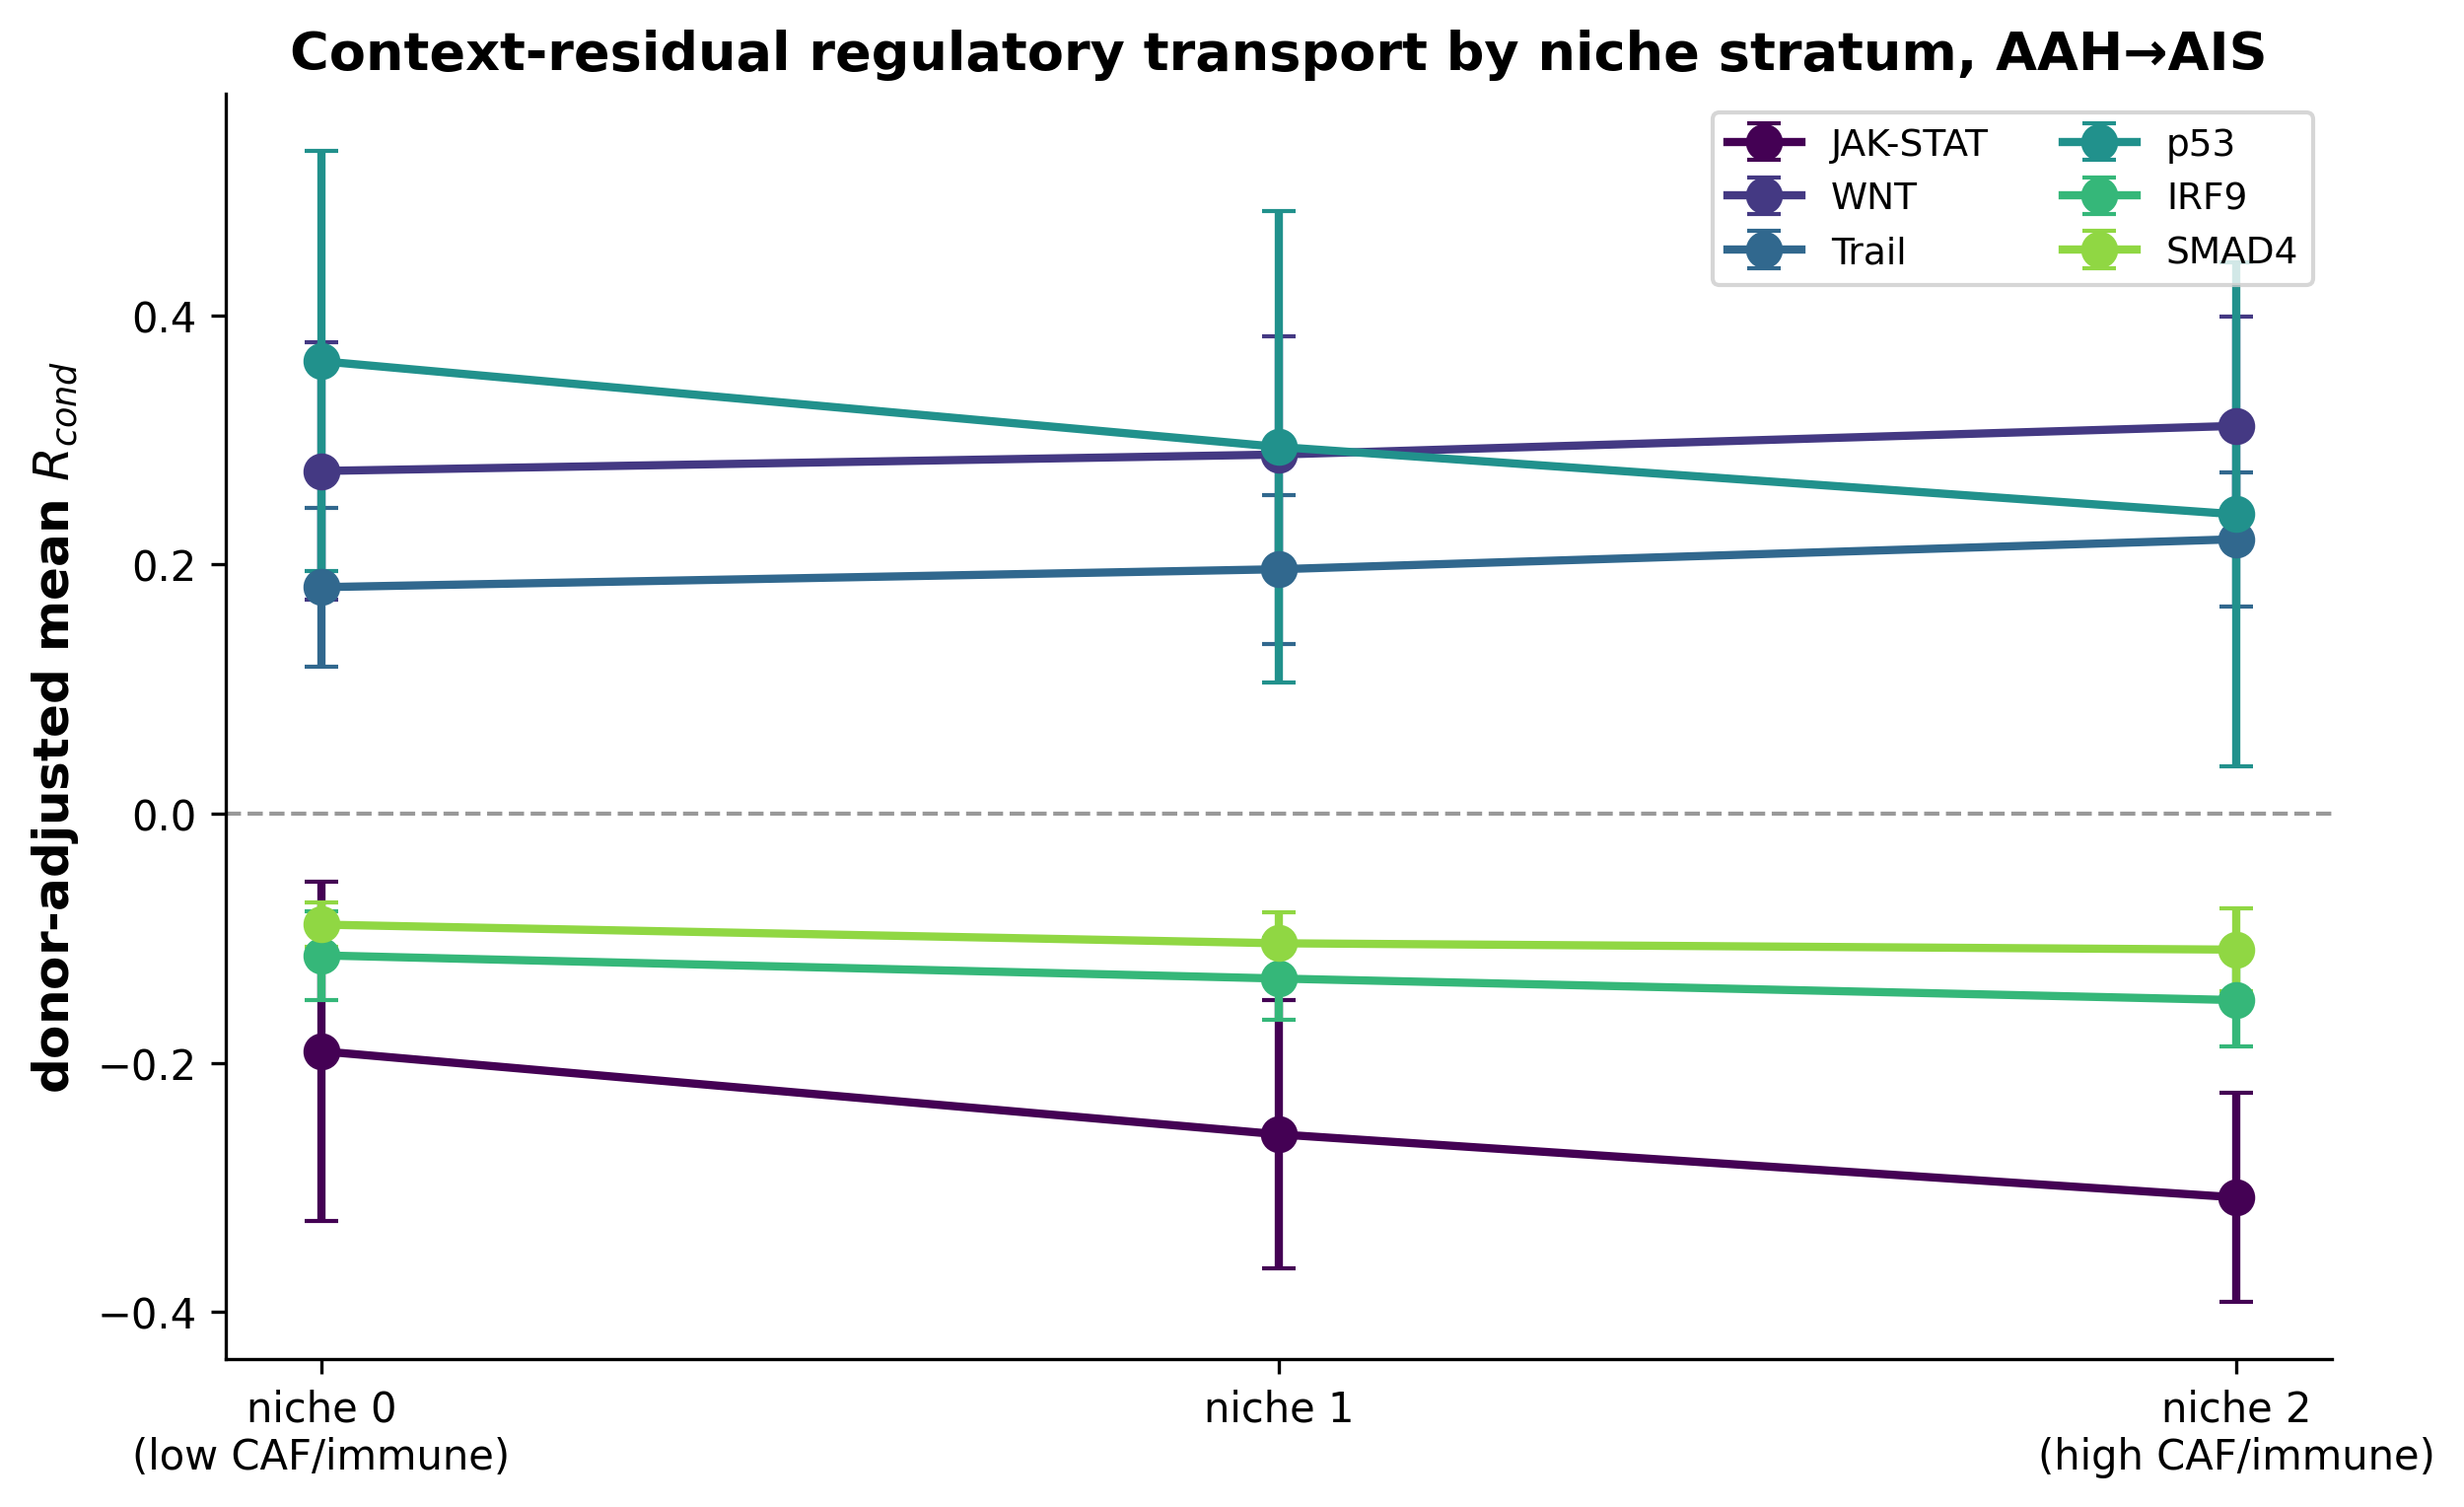
\includegraphics[width=0.85\textwidth]{figures/rcond_niche_gradient_AAH_AIS.png}
  \caption[Context-residual transport by niche stratum, AAH$\rightarrow$AIS]{Donor-adjusted mean $R_{\text{cond}}$ for the leading stable programs across the three conditional-stratified niche strata (stratum~0 low to stratum~2 high CAF/immune density) on the AAH$\rightarrow$AIS edge. Whiskers are 95\% confidence intervals over the five patient-held-out folds. JAK-STAT redirection deepens and WNT/TRAIL rise toward the CAF/immune-dense stratum, while p53 declines; the gradients are monotonic but modest, indicating regulatory redirection graded by coarse ecological stratum rather than switched by a single niche identity.}
  \label{fig:niche_gradient}
\end{figure}

\section{The ecological variation that would carry progression signal is specimen-scale, not receiver-local}
\label{sec:results-scale}

The dominance of specimen-level ecology over cell-resolved niche in the falsification ladder (Section~\ref{sec:results-ladder}) is explained by the spatial scale at which context varies. A variance decomposition of the local composition features shows that the large majority of variance in macrophage, fibroblast, CAF, and immune abundance is receiver-local (within-slide: $91\%$ for alveolar macrophage, $87\%$ for total macrophage, $90\%$ for fibroblast, $85\%$ for the CAF fraction), with only a modest between-patient component ($8$--$15\%$) and a negligible between-stage component ($<1\%$; Fig.~\ref{fig:variance_partition}). Because so much ecological variation is local and stage-invariant, a cell-resolved context feature carries substantial noise relative to its progression-aligned signal, which is consistent with the ladder finding that resolving local niche did not separate cleanly from specimen-level ecology.

The spatial organization of that ecology, however, is neither random nor static across progression. Computing spatial autocorrelation on the full-cohort composition features within each tissue section (Moran's~$I$, $k=15$ nearest-neighbor graph, $55$ sections spanning $787{,}816$ spots; all $330$ section-by-feature tests are individually significant at $P_{\text{norm}}<0.05$), every composition feature is positively autocorrelated at every stage, confirming that the microenvironment is spatially structured rather than well-mixed. Malignant-cell density is the feature whose spatial clustering changes most across the precursor sequence: mean Moran's~$I$ rises monotonically from $0.234 \pm 0.025$ at AAH ($n=11$ sections) to $0.458 \pm 0.070$ at AIS ($n=14$) to $0.701 \pm 0.034$ at invasive disease ($n=30$; Spearman $\rho = 0.673$ between section-level Moran's~$I$ and stage order, $P = 1.8\times10^{-8}$; Kruskal--Wallis $H = 24.6$, $P = 4.6\times10^{-6}$; AAH versus invasive Mann--Whitney $P = 3.6\times10^{-6}$). The corresponding Getis--Ord Gi* hot-spot fraction for malignant density nearly doubles across the same sequence ($0.118 \rightarrow 0.131 \rightarrow 0.234$; $\rho = 0.64$, $P = 1.2\times10^{-7}$). CAF and immune fractions show the same directional increase toward invasion ($0.426 \rightarrow 0.545$ and $0.416 \rightarrow 0.503$), whereas macrophage autocorrelation is high but stage-flat ($0.443 \rightarrow 0.499 \rightarrow 0.467$): the ecological compartments most implicated in the context residual are spatially organized within every specimen but only weakly graded by stage. This local macrophage compartment is, however, quantitatively coupled to the context residual on the authoritative full-cohort table: in a donor-random-intercept mixed model of per-receiver $R_{\text{cond}}$ on local macrophage abundance ($66{,}834$ receivers, $10$ donors), the inflammatory programs JAK-STAT and NF$\kappa$B increase their context effect with macrophage density (JAK-STAT $+0.043$, NF$\kappa$B $+0.039$ per SD; both positive across the cohort), consistent with the pre-registered hypothesis that a proinflammatory macrophage niche is associated with context-driven regulatory redirection. The full per-program model, and the finding that stage-level marginal composition itself does not separate the two stages at the donor level, are given in Appendix~\ref{sec:app-c-il1b-provisional}. The stage trends in autocorrelation are summarized in Figure~\ref{fig:moran_getis}, and the spatial organization of malignant clustering is illustrated for representative AAH and AIS sections in Figure~\ref{fig:spatial_autocorr_maps}.

% NOTE: the requested third panel (figures/spatial/moran_by_stage_AAH_AIS.pdf) is intentionally
% OMITTED. Its staged content plots only two stages (AAH, AIS; no invasive), Moran's I in the range
% -0.025 to +0.015 with immune_fraction negative, and malignant density DECREASING from AAH to AIS --
% which contradicts the monotonic 0.234 -> 0.458 -> 0.701 trend and "every feature positively
% autocorrelated" claim in the prose above. Its generator (crrt/viz/spatial_figures.py:
% plot_moran_by_stage) pools all spots of a stage into one spatial graph, mixing coordinates across
% sections and destroying autocorrelation; it is superseded by the memory-safe per-section recompute
\begin{figure}[htbp]
  \centering
  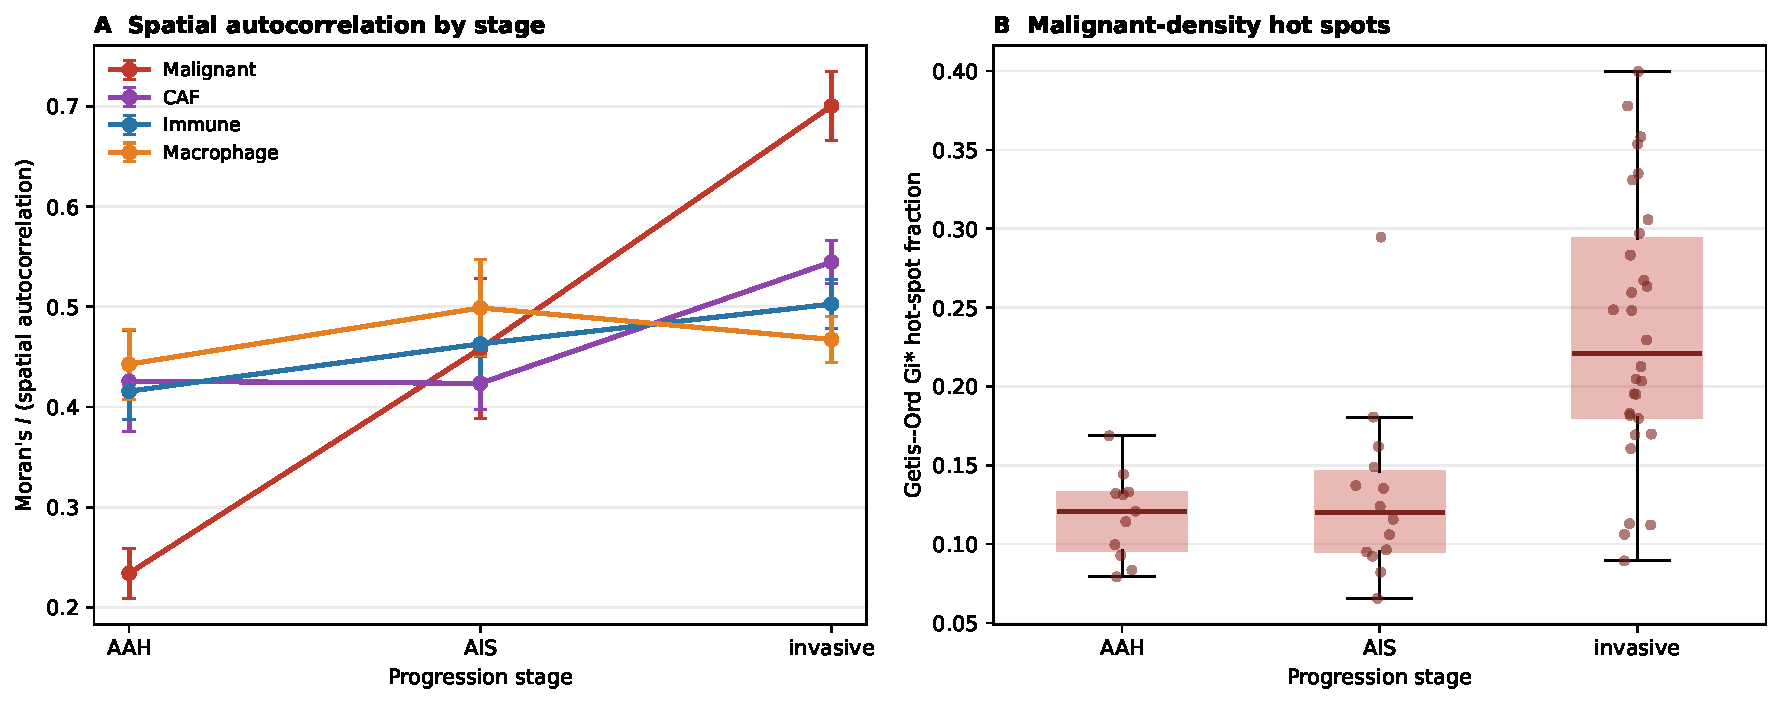
\includegraphics[width=0.95\textwidth]{figures/spatial/moran_getis_by_stage.pdf}
  \caption[Spatial autocorrelation of composition by stage]{Section-level spatial autocorrelation
  across the precursor sequence (55 sections). \textbf{(a)}~Mean Moran's~$I$ per compartment; malignant
  density rises steeply ($0.23\!\rightarrow\!0.70$) while macrophage stays stage-flat. \textbf{(b)}~
  Getis--Ord Gi* hot-spot fraction for malignant density, per section. Whiskers/boxes are across
  sections.}
  \label{fig:moran_getis}
\end{figure}

\begin{figure}[htbp]
  \centering
  \begin{subfigure}[t]{0.48\textwidth}
    \centering
    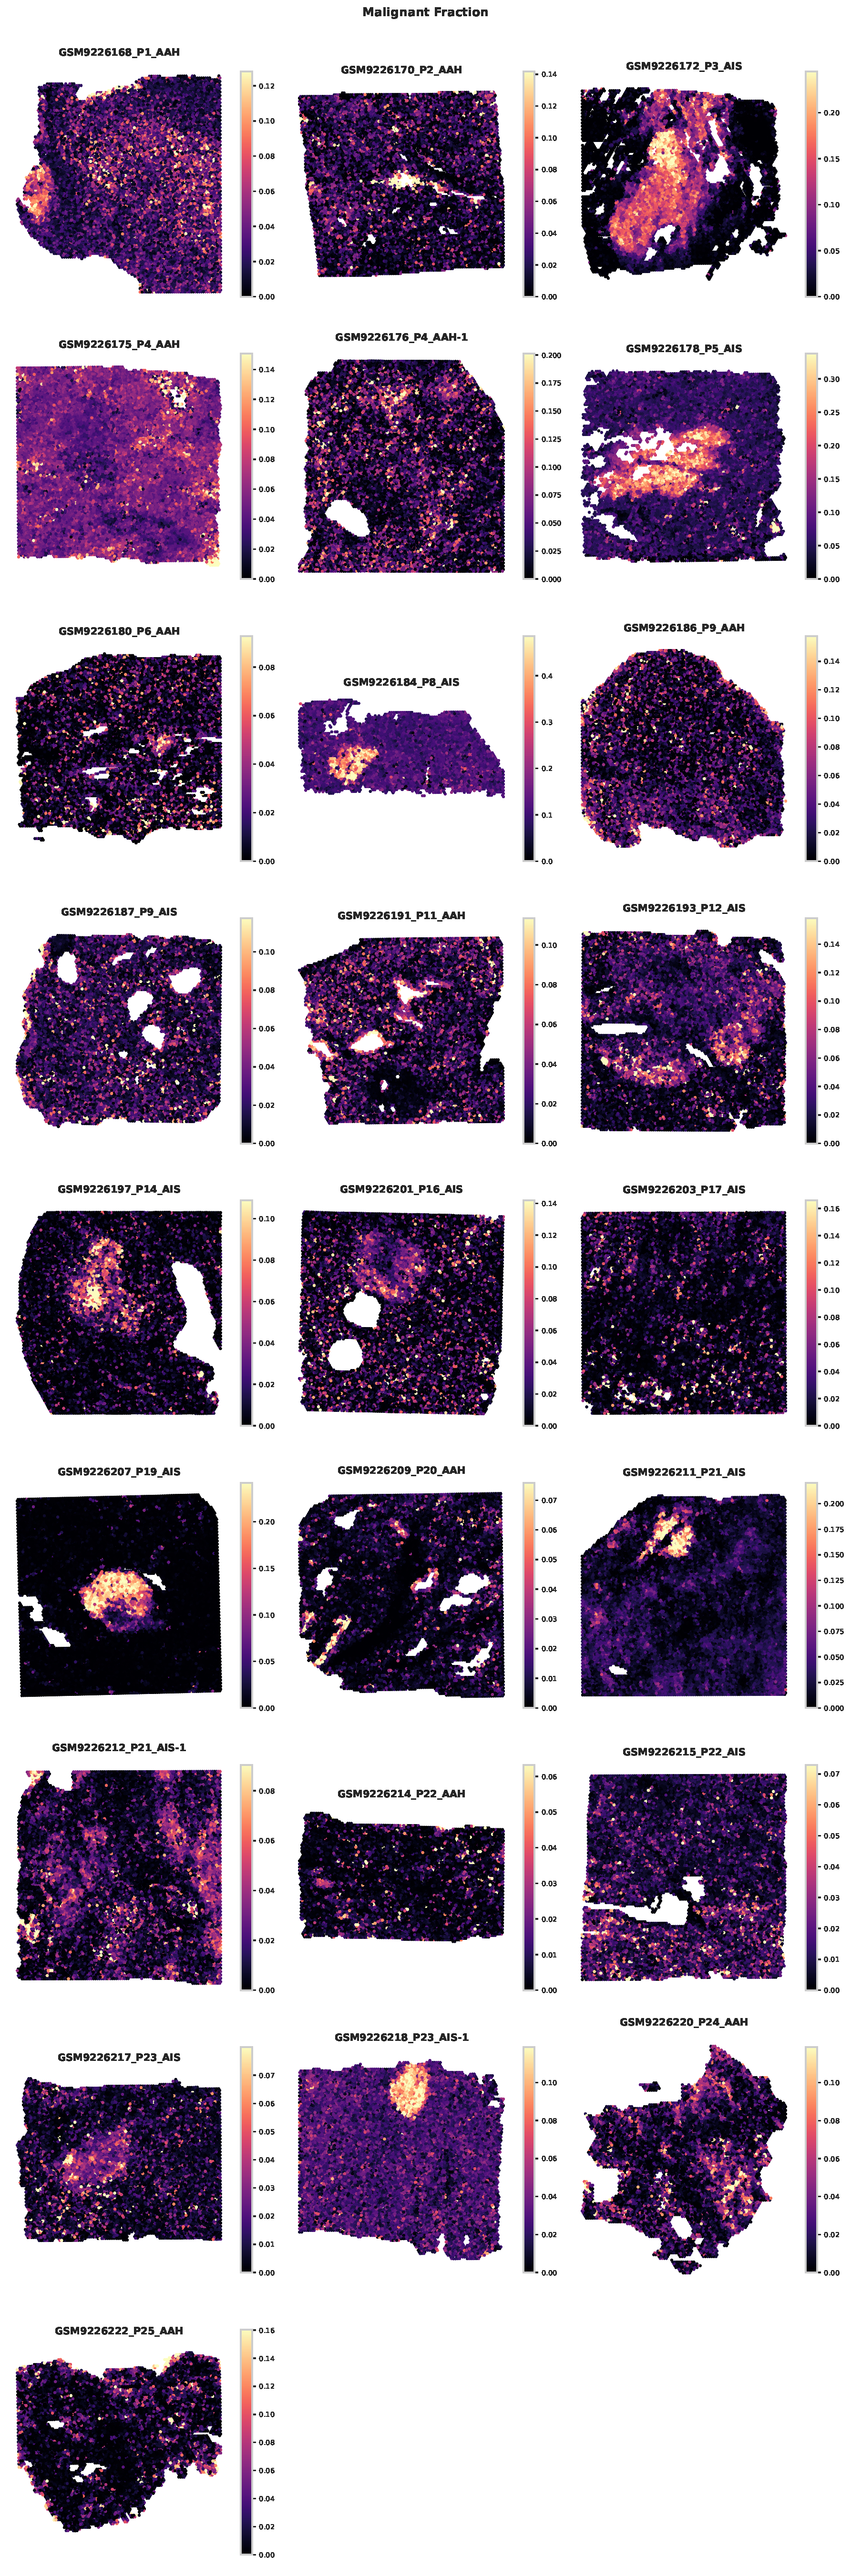
\includegraphics[width=\textwidth]{figures/spatial/spatial_malignant_fraction_AAH_AIS.pdf}
    \caption{Malignant-cell fraction per spot}
    \label{fig:spatial_autocorr_malig}
  \end{subfigure}\hfill
  \begin{subfigure}[t]{0.48\textwidth}
    \centering
    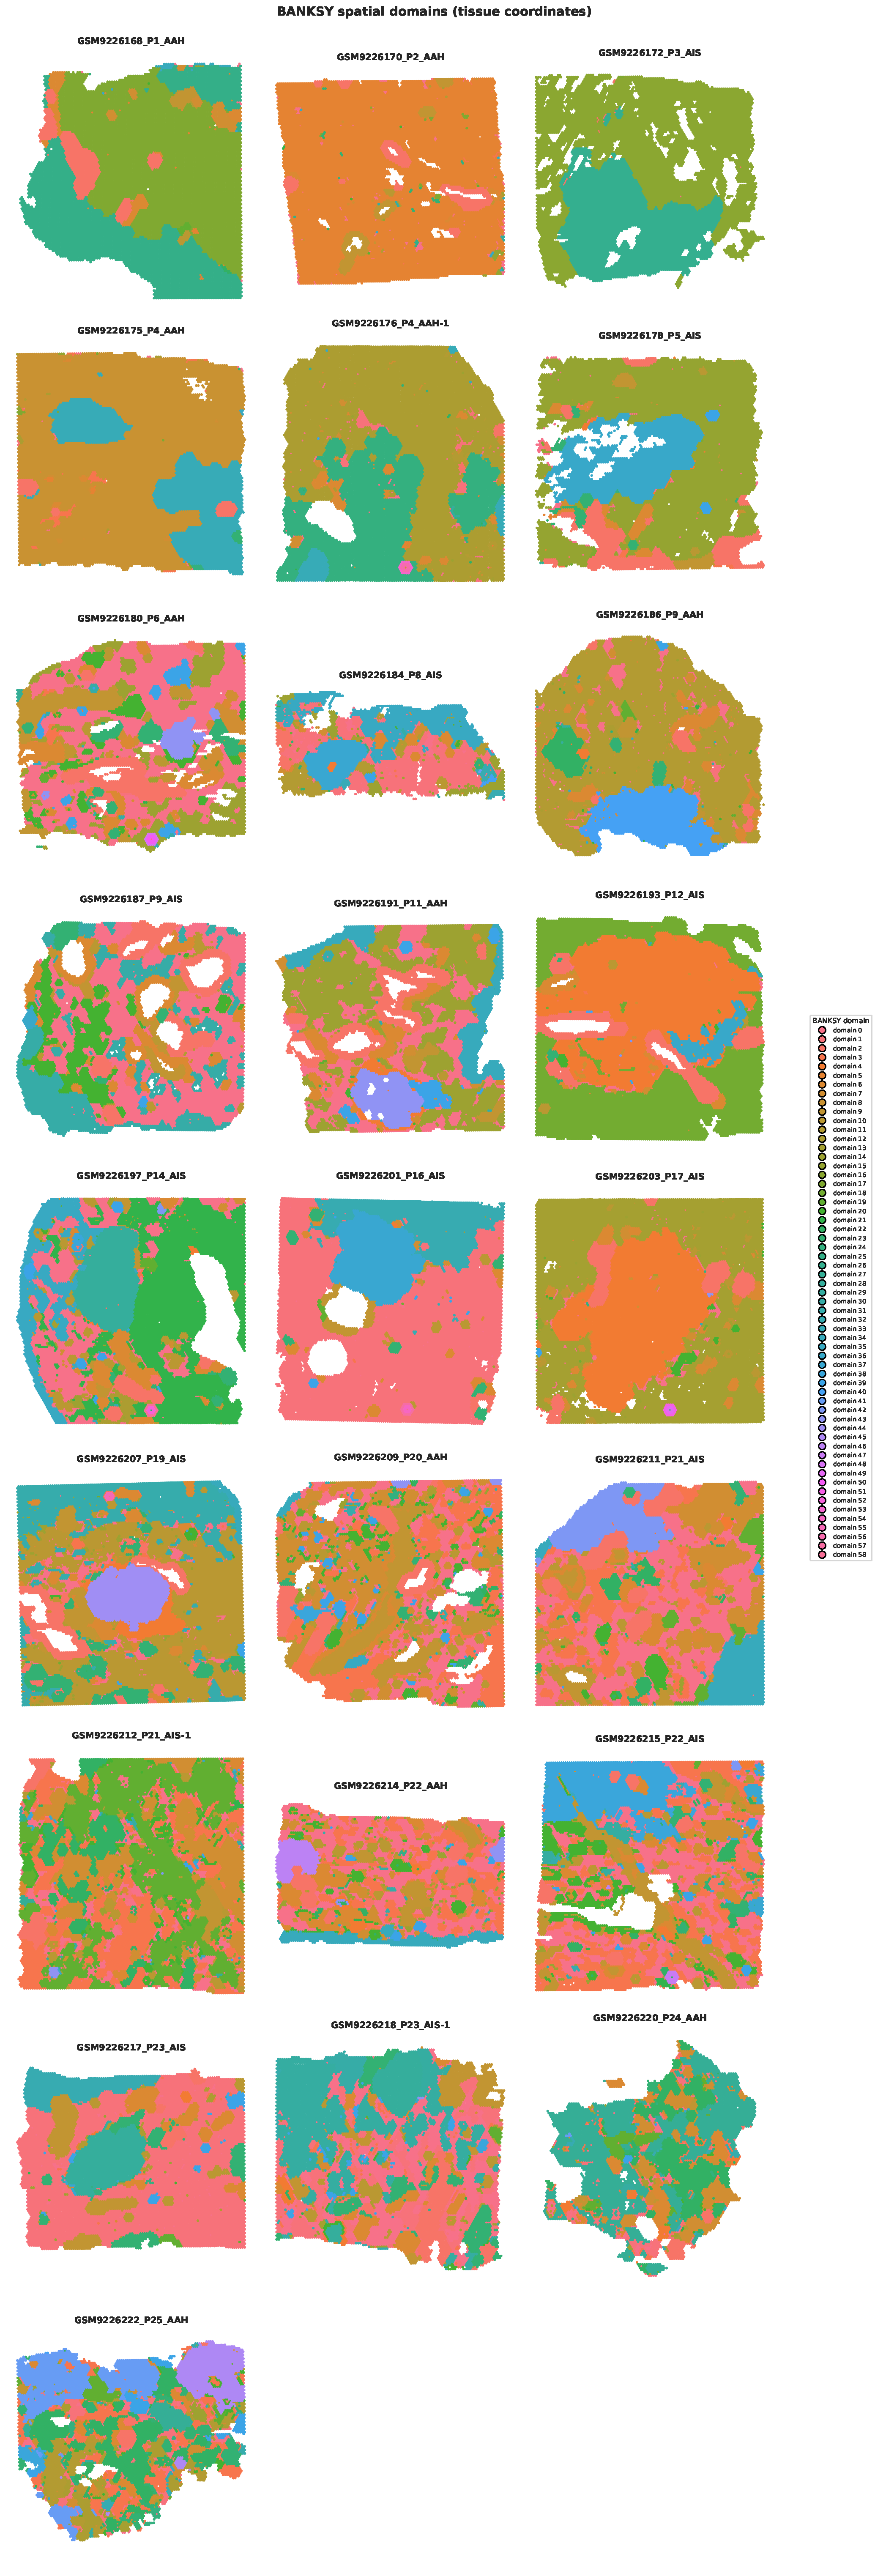
\includegraphics[width=\textwidth]{figures/spatial/banksy_domain_map_AAH_AIS.pdf}
    \caption{BANKSY spatial domains}
    \label{fig:spatial_autocorr_banksy}
  \end{subfigure}
  \caption[Spatial organization of the AAH and AIS microenvironment]{Microenvironment across the AAH
  and AIS Visium sections (tissue coordinates; one sub-panel per section). \textbf{(a)}~Local malignant
  fraction is concentrated in focal, contiguous foci, more pronounced in several AIS sections.
  \textbf{(b)}~BANKSY domains partition each section into spatially coherent microenvironments,
  confirming the composition features are spatially structured. These descriptive maps illustrate the
  spatial structure quantified in the text (the monotonic rise in malignant Moran's~$I$ and positive
  within-section autocorrelation); they are not themselves a statistical test.}
  \label{fig:spatial_autocorr_maps}
\end{figure}


These two observations---a stratum gradient significant against a within-donor null, and a variance
decomposition placing $85$--$96\%$ of local ecological variance at the receiver scale and
stage-invariant---are not in tension once their referents are distinguished. The gradient is a
statement about \emph{parameter structure}: across roughly $10^{4}$ receivers, a small but systematic
ordering of per-program residuals by coarse ecological stratum is detectable, and the permutation null
confirms it is not carried by between-donor composition. The variance decomposition is a statement
about \emph{how much progression-aligned ecological signal is available to an endpoint metric}: if the
overwhelming majority of variance in the same composition features is local and stage-invariant, then a
receiver-resolved context feature supplies a small, reproducible ordering embedded in a large amount of
stage-orthogonal variation. A reproducible effect of that magnitude is exactly what fails to move a
distributional endpoint distance while remaining detectable in a per-program contrast. The two results
therefore describe one regime from two directions: context redirection is real, graded, and small, and
it is small in precisely the way the ecological scale of the measurement predicts.

\begin{figure}[htbp]
  \centering
  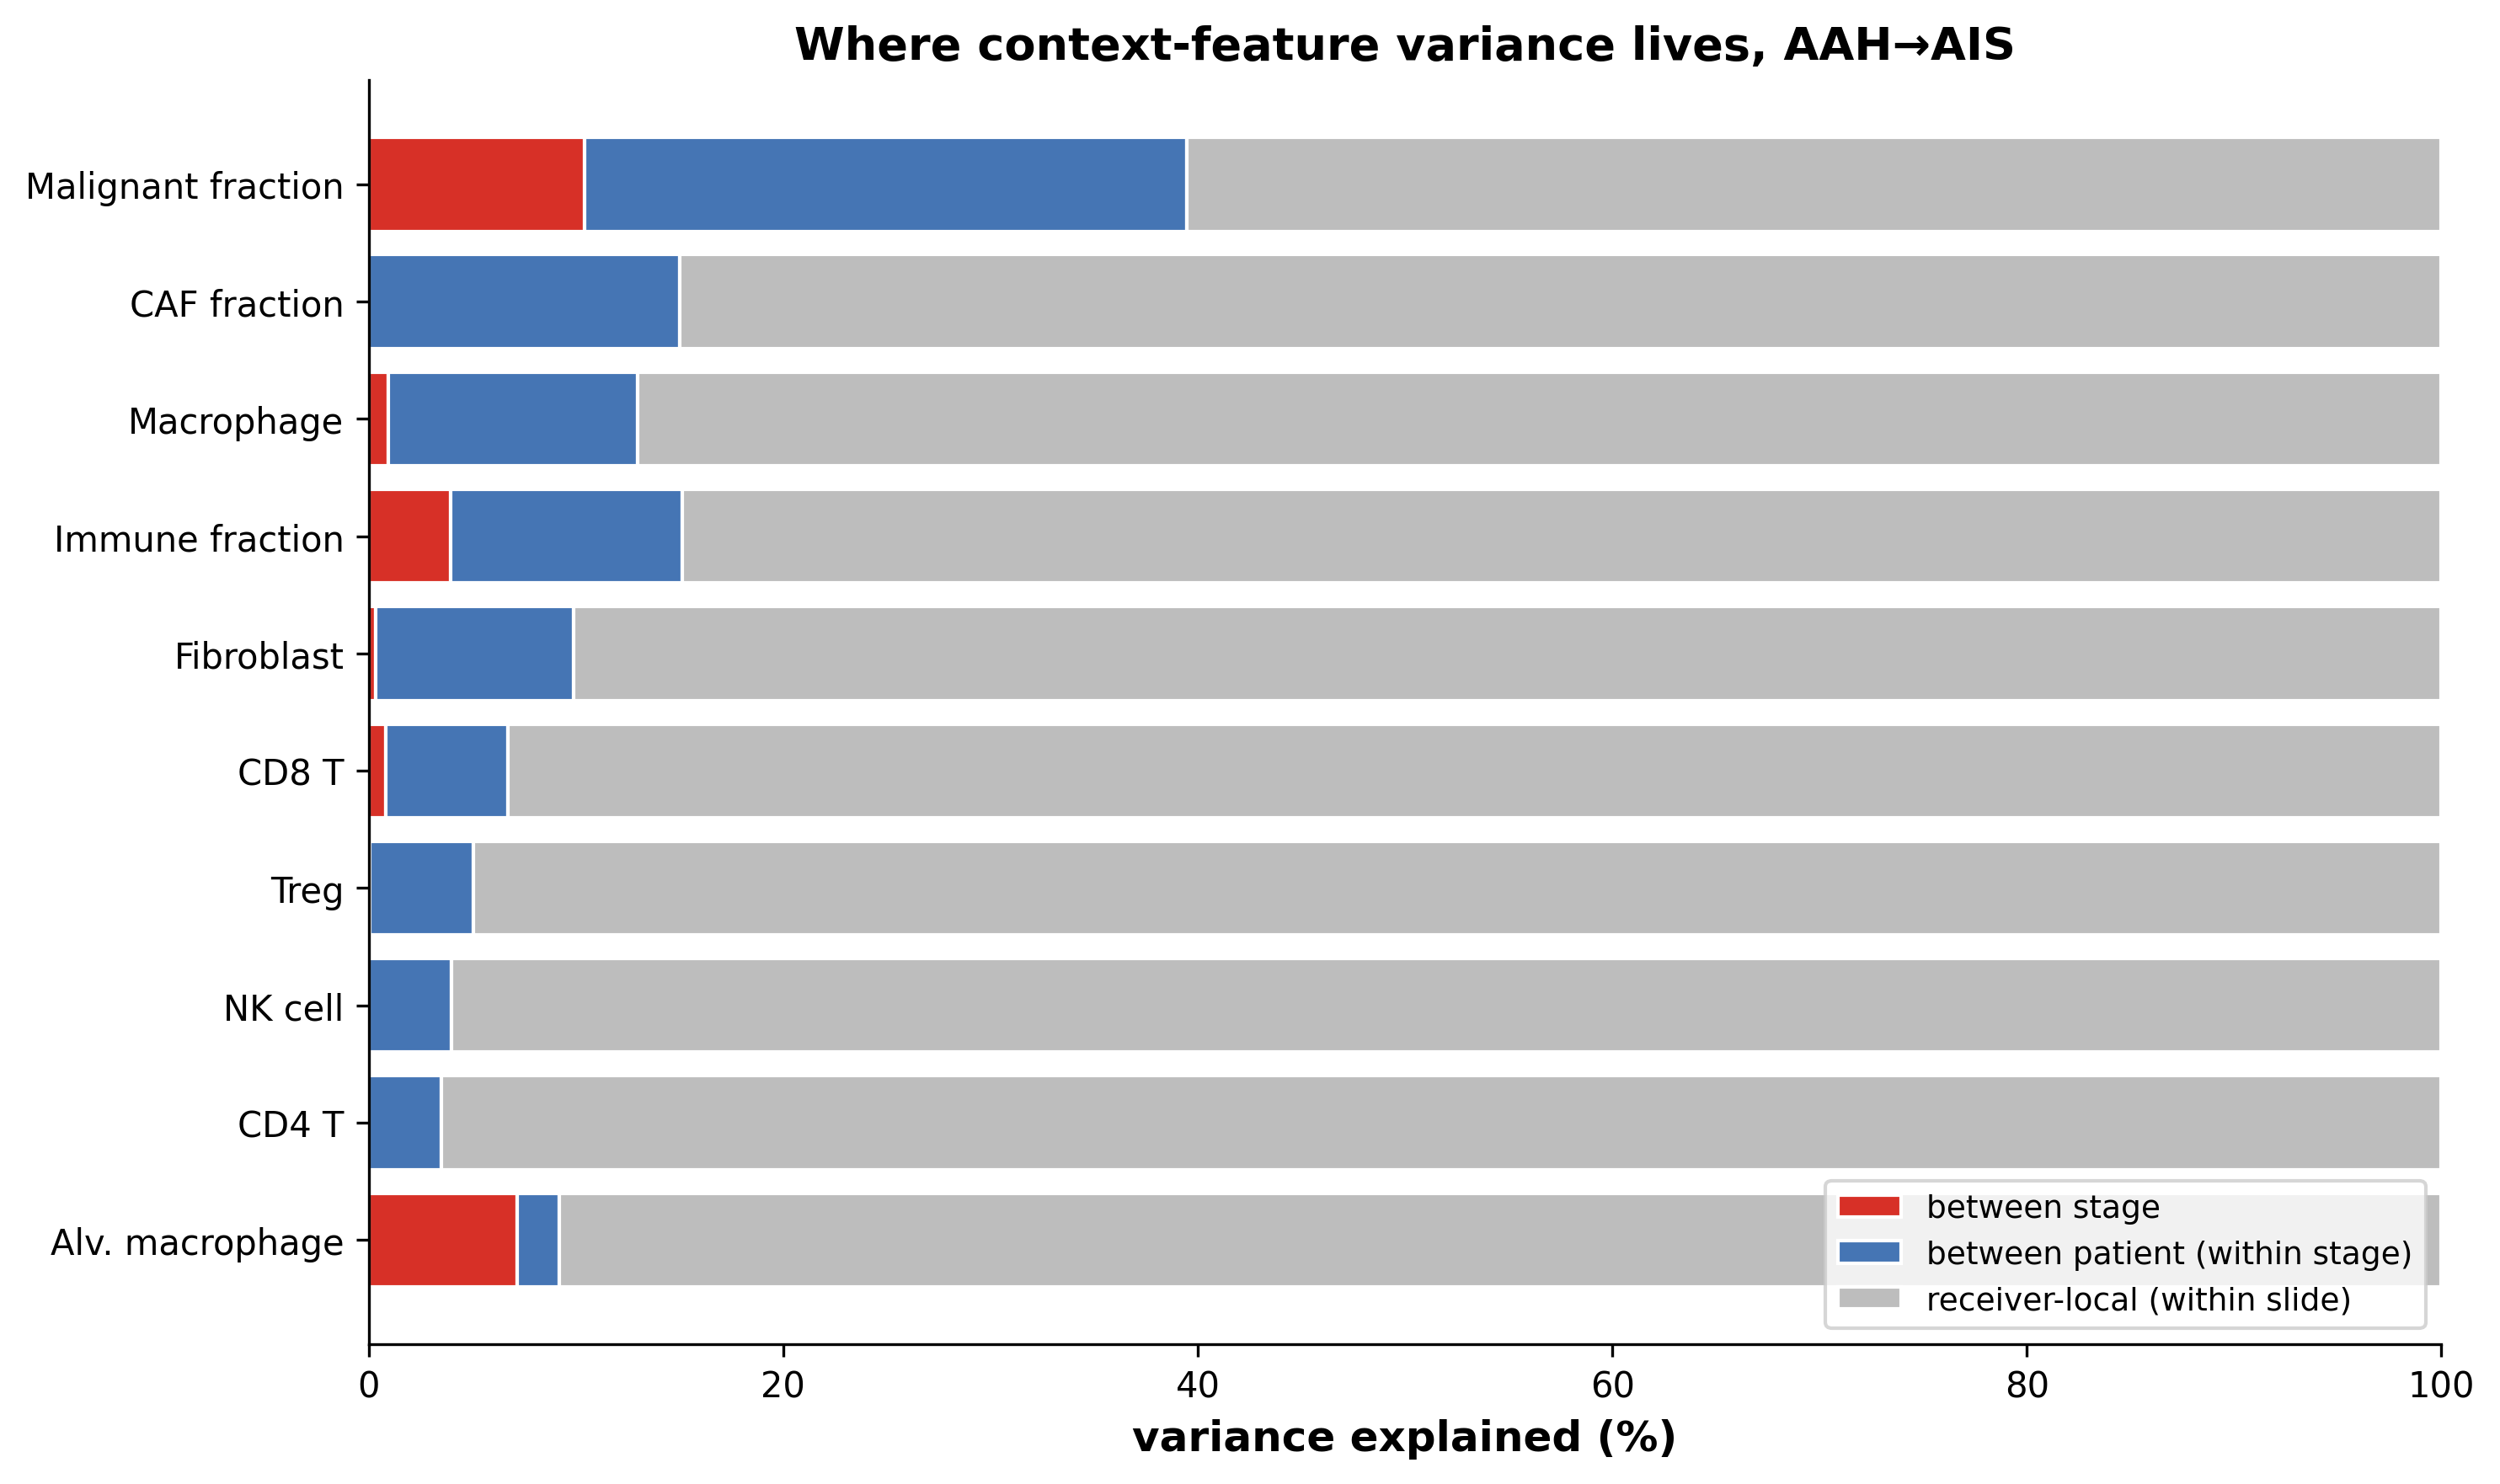
\includegraphics[width=0.85\textwidth]{figures/variance_partition_AAH_AIS.png}
  \caption[Variance decomposition of local context features]{Decomposition of variance in each local composition feature into between-stage (red), between-patient within stage (blue), and receiver-local within-slide (grey) components, on the AAH$\rightarrow$AIS spatial cohort. The receiver-local component dominates every feature ($85$--$96\%$; nested variance decomposition on the authoritative full-cohort context table), the between-stage component is small ($<1\%$), and the between-patient component is modest ($8$--$15\%$). High receiver-local variance with low between-stage variance is the ecological-scale explanation for why cell-resolved niche context did not outperform specimen-level ecology in the falsification ladder.}
  \label{fig:variance_partition}
\end{figure}

\section{Transport geometry, decomposition credibility, and sensitivity to modeling choices}
\label{sec:credibility}

Intrinsic regulatory state carries a stage signal that does not transfer across patients, which is the motivation for patient-held-out evaluation throughout this work. Under \emph{donor}-held-out cross-validation a supervised classifier of the 773 regulatory self-features separates AAH from AIS at a mean area under the receiver-operating-characteristic curve of $0.419$ (SD $0.110$; per-fold $0.27$ to $0.61$; 89{,}172 epithelial cells across the 18 donors carrying either stage---a larger set than the $78{,}400$ edge-bridging \emph{receivers} used for transport in Table~\ref{tab:edge_support}, because the classifier draws on all AAH- and AIS-labeled epithelium rather than only donors that bridge the edge; Figure~\ref{fig:self-only-roc})---approximately $1.6$ standard errors below $0.5$, that is, below chance out of sample. A pooled classifier that does not hold out donors reaches AUC $0.835$, but this edge has only two donors that contribute both stages, so donor identity is largely confounded with stage and the pooled value cannot be attributed to stage-discriminative signal. Classifying stage \emph{inside} individual donors that contribute both stages holds donor identity constant instead, so any above-chance discrimination there is stage biology rather than donor recognition. On the earlier Normal$\rightarrow$AAH edge, which has eight such shared donors, within-donor classification is above chance in every donor and averages AUC $0.833$ (SD $0.103$; per-donor range $0.686$ to $0.975$; donors contributing $672$ to $21{,}457$ cells per class), and the two donors that bridge the AAH$\rightarrow$AIS edge give a concordant $0.891$ and $0.744$. Intrinsic regulatory state therefore encodes the stage distinction independent of patient identity; what fails is cross-patient transfer, not the representation---a self-only classifier does not generalize to unseen patients (donor-held-out AUC $0.419$), which is why every estimate in this chapter is patient-held-out.

The transport geometry is identifiable but the grey-box decomposition is borderline, and both facts are reported. The normalized matching-stability diagnostic $D_N$ favors the pathway-plus-transcription-factor regulatory geometry used for estimation, and the pathway subspace is the most stable block ($D_N$ per feature $0.050$ over 14 pathways versus $0.0049$ over 759 transcription factors), so the estimated dynamics are identifiable on the geometry over which transport was defined (full $D_N$ diagnostics in Appendix~\ref{sec:app-c-coupling}). The credibility gate $D_{\rho}$---the ratio of neural-residual velocity to structured-algebra velocity in the fitted full field---is $0.965$ on average (range $0.922$ to $1.008$ over the five folds), with four of five folds credible ($D_{\rho} \leq 1$, regime \textsc{structured\_neural}) and fold~2 residual-dominated ($D_{\rho} = 1.008$). The interpretable regulatory terms therefore carry velocity of comparable magnitude to the neural residuals in the joint fit, rather than dominating it; the per-program $R_{\text{cond}}$ readouts of Sections~\ref{sec:stable} and~\ref{sec:invasion-signature} are interpretable to that extent, and the ablation ladder (Table~\ref{tab:ladder}) shows the structured algebra cannot reproduce the transport on its own ($\text{structured\_only} = 2621.22$ versus $123.65$ for the full field). The decomposition is thus credible but not residual-free, and the per-program attribution is bounded by that ceiling.

The fitted transport is also increasingly non-equilibrium along the progression axis. A Helmholtz decomposition of the learned field partitions its velocity into a gradient (equilibrium) and a rotational (non-equilibrium) component; the rotational fraction rises from $0.48$ on the preinvasive AAH$\rightarrow$AIS edge to $0.77$ on the AIS$\rightarrow$invasive edge, and is lowest ($0.26$) on the underpowered PanIN edge. The invasive transition is therefore the most strongly non-gradient---consistent with a directed, cycle-like progression flow rather than relaxation toward a fixed point---while the addition of context changes this fraction only marginally on every edge (self-only versus full-field difference $\leq 0.011$), so the non-equilibrium character is a property of the intrinsic progression field rather than of the niche-gated term. The fitted field is shown in Figure~\ref{fig:fitted-velocity-field}, and the niche-gated component itself, $v_{\text{full}}-v_{\text{self}}$, is rendered directly as the context difference field for both LUAD edges in Figure~\ref{fig:context_diff_field}.

\begin{figure}[htbp]
  \centering
  \begin{subfigure}{\textwidth}
    \centering
    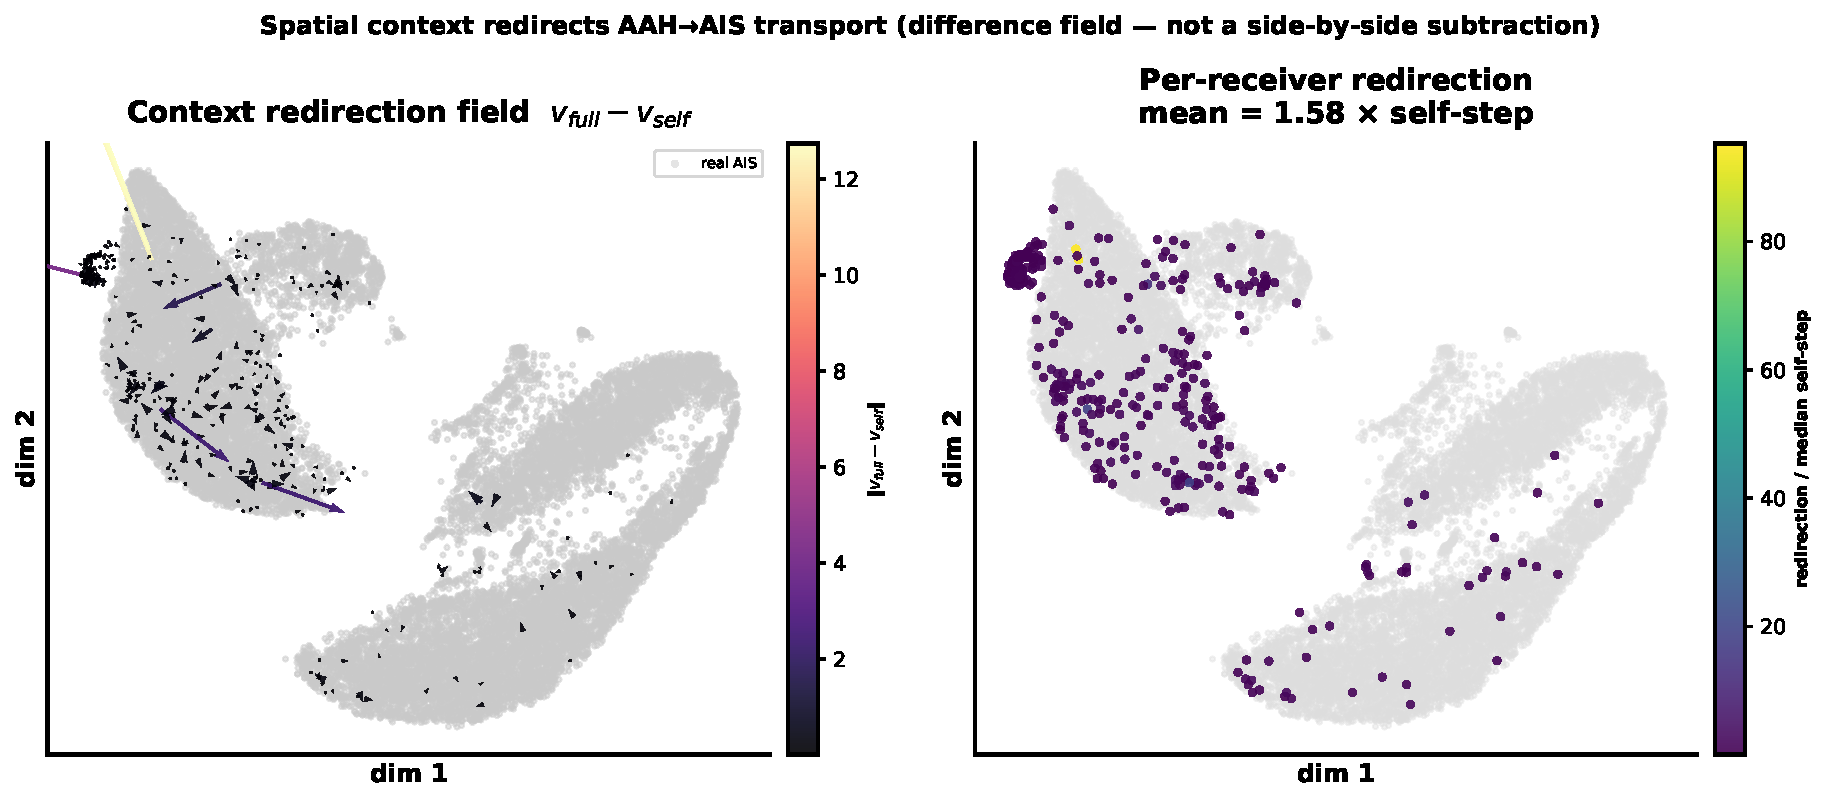
\includegraphics[width=0.98\textwidth]{figures/ude_result/context_difference_field_AAH_AIS.pdf}
    \caption{AAH$\rightarrow$AIS (preinvasive edge). Left: the context redirection vector field, an arrow $v_{\text{full}}-v_{\text{self}}$ at each source receiver; right: the same receivers recoloured by redirection magnitude relative to the median self-only step.}
    \label{fig:context_diff_field-aah}
  \end{subfigure}

  \vspace{0.7em}

  \begin{subfigure}{\textwidth}
    \centering
    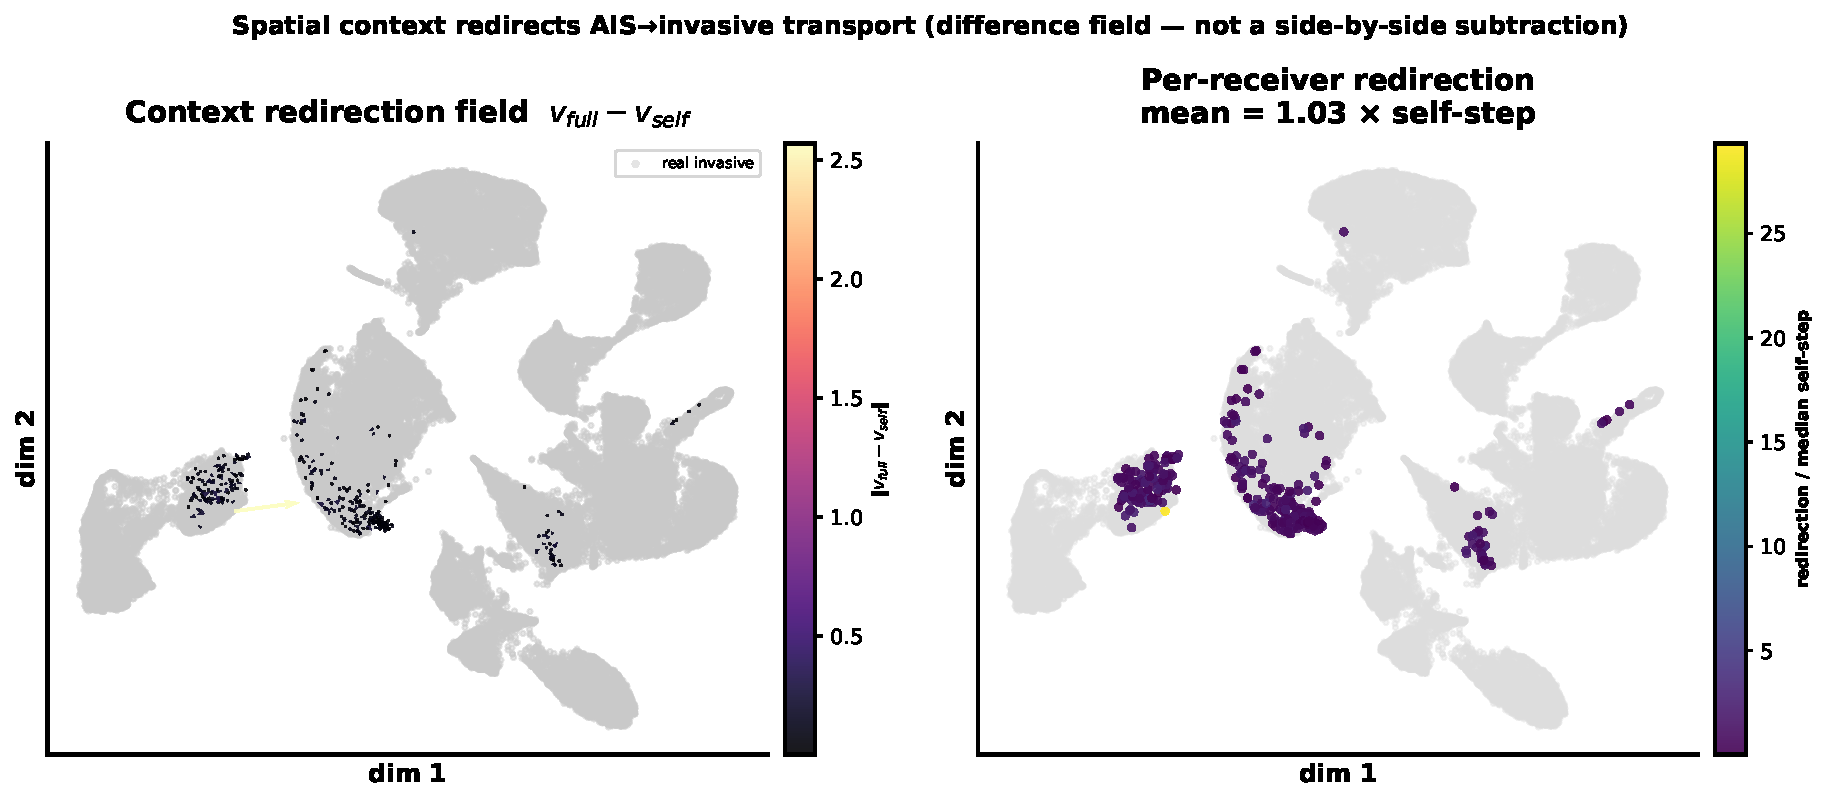
\includegraphics[width=0.98\textwidth]{figures/ude_result/context_difference_field_AIS_invasive.pdf}
    \caption{AIS$\rightarrow$invasive edge, same two-panel layout.}
    \label{fig:context_diff_field-inv}
  \end{subfigure}
  \caption[Context difference field, both LUAD edges]{The niche-gated transport component
  $v_{\text{full}}-v_{\text{self}}$ for (a)~the preinvasive and (b)~the invasion edge, projected into
  the regulatory embedding (arrows, coloured by magnitude; grey points are target-stage receivers).
  The redirection is spatially coherent but small relative to the self-only step, consistent with the
  $\leq 0.011$ context shift in rotational fraction. This is an illustrative view; per-program
  significance is quantified by $R_{\text{cond}}$ (Fig.~\ref{fig:forest}).}
  \label{fig:context_diff_field}
\end{figure}


\begin{figure}[htbp]
  \centering
  \begin{subfigure}{\textwidth}
    \centering
    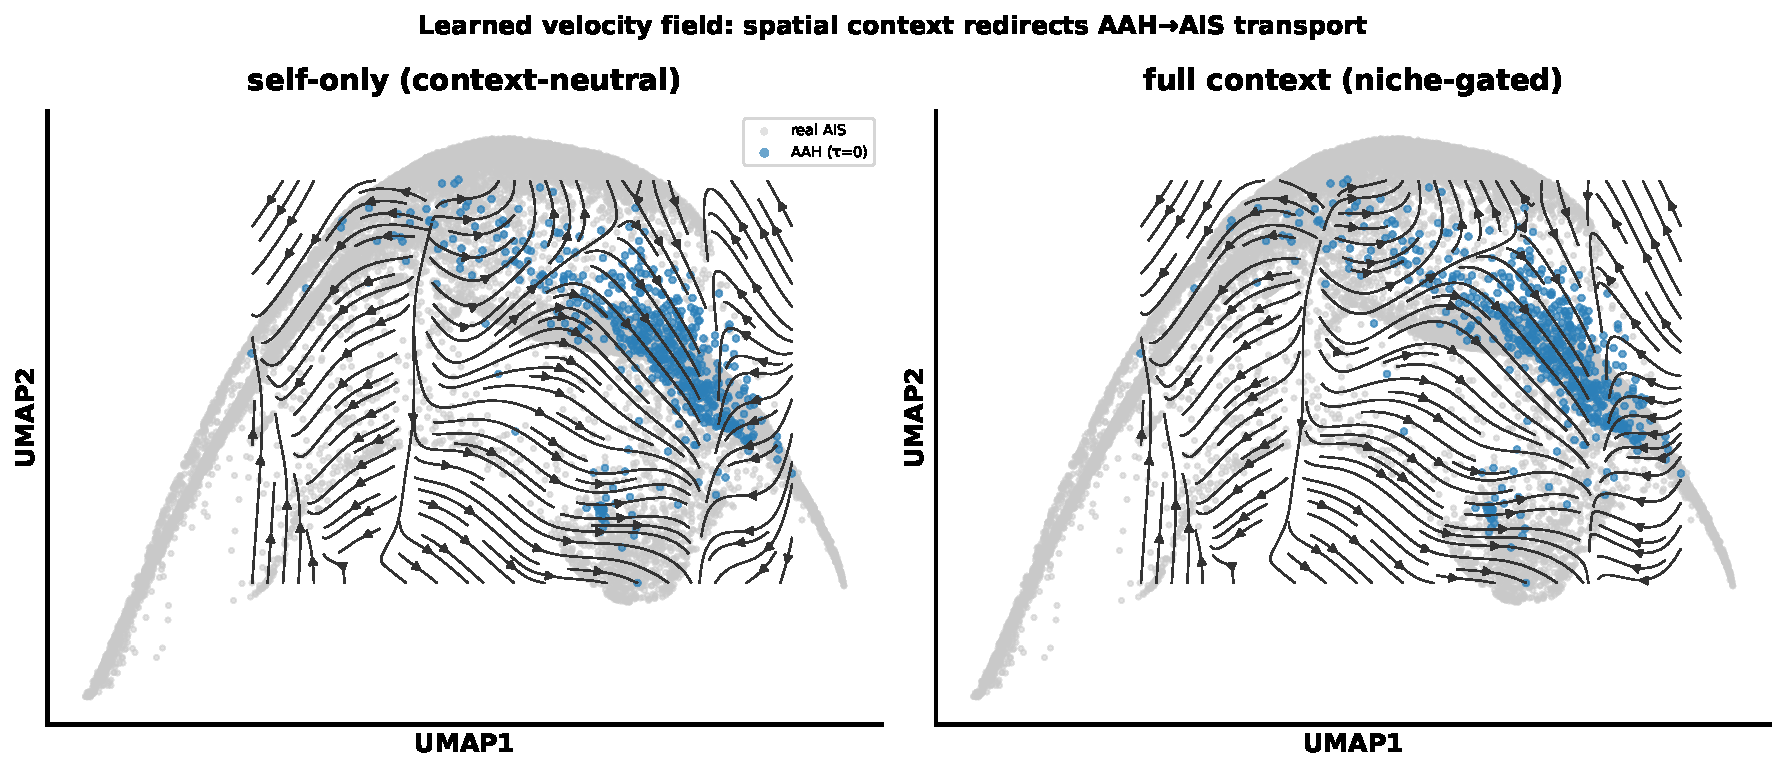
\includegraphics[width=\textwidth]{figures/dynamics/velocity_streamplot_AAH_AIS.pdf}
    \caption{Preinvasive edge (AAH$\rightarrow$AIS).}
    \label{fig:fitted-velocity-field-aah}
  \end{subfigure}\\[0.8em]
  \begin{subfigure}{\textwidth}
    \centering
    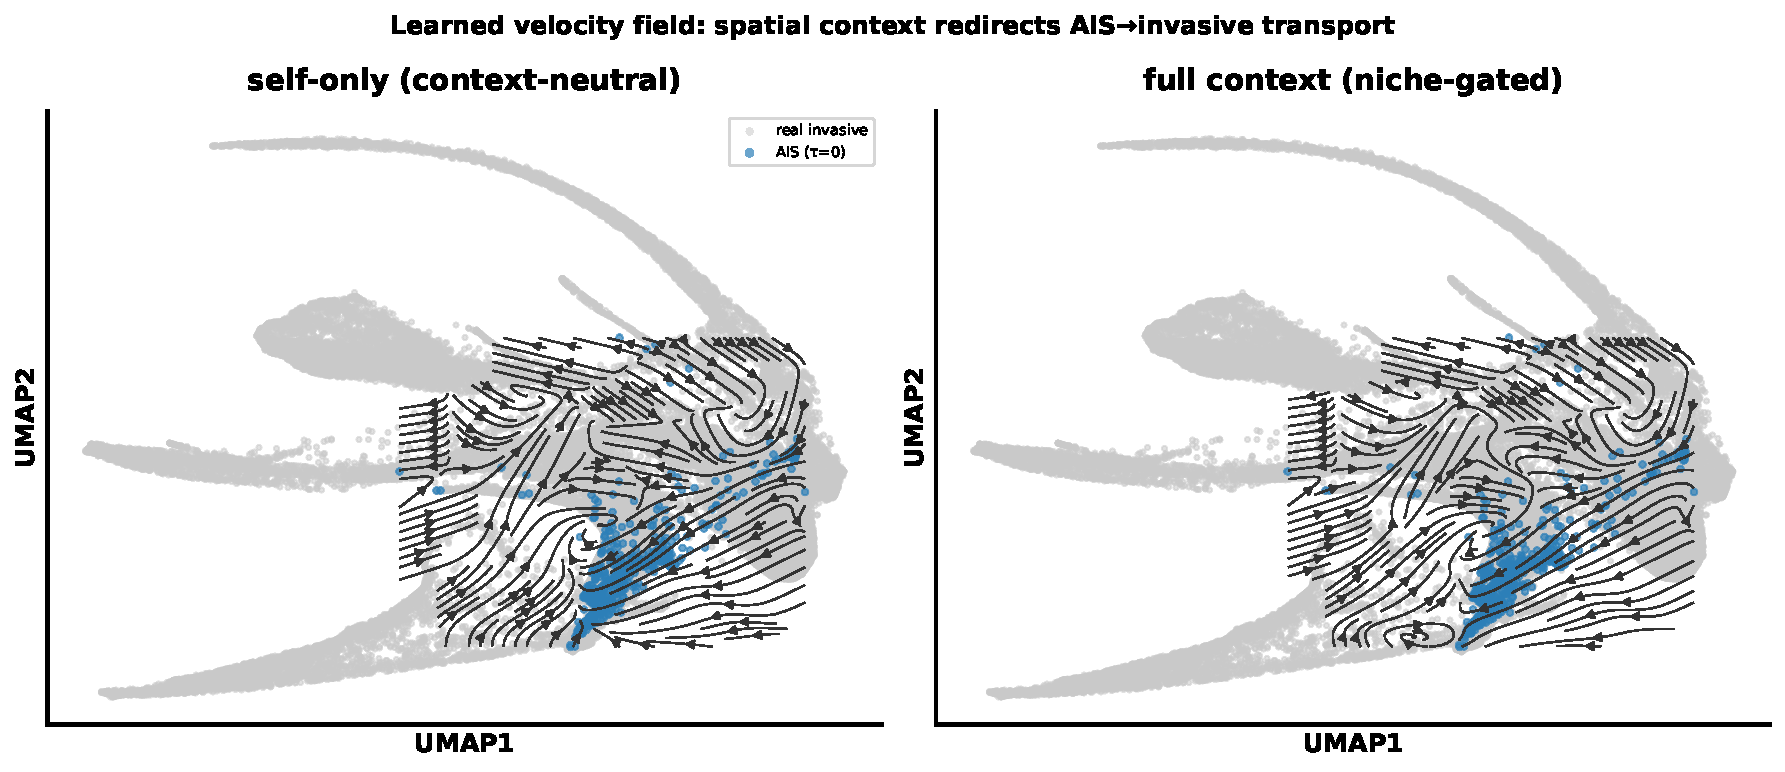
\includegraphics[width=\textwidth]{figures/dynamics/velocity_streamplot_AIS_invasive.pdf}
    \caption{Invasion edge (AIS$\rightarrow$invasive).}
    \label{fig:fitted-velocity-field-ais}
  \end{subfigure}
  \caption[Fitted regulatory velocity field along the progression axis]{Learned CRRT-UDE transport
  as streamlines on the pooled receiver UMAP, self-only (context-neutral) beside full-context
  (niche-gated), over source receivers at $\tau=0$ (blue) and target receivers (grey); colour and width
  encode field speed. \textbf{(a)}~preinvasive AAH$\rightarrow$AIS and \textbf{(b)}~AIS$\rightarrow$invasive.
  The fields are directed rather than relaxational, and the two streamline sets are near-indistinguishable
  on both edges---the niche-gated term redirects transport only modestly, which is why the redirection is
  shown directly in Fig.~\ref{fig:context_diff_field} rather than read off by eye.}
  \label{fig:fitted-velocity-field}
\end{figure}


One further reproducibility check anchors the stable set at the donor level: every program
classed STABLE on the AAH$\rightarrow$AIS edge holds its sign not only across the five patient-held-out
folds but also under leave-one-donor-out resampling (sign consistency $1.0$), so no single specimen
drives the stable count. Together with the transport-geometry and grey-box diagnostics above, the two
load-bearing conclusions of this chapter are robust to estimation choices in different ways: the
positive result (a reproducible program-level residual) is supported by donor-level and cross-fold
reproducibility, while the negative result (its failure to resolve at the receiver-local scale) is the
more thoroughly stressed of the two---it holds across all five folds, both LUAD edges, a specimen-level
average, a stratum-matched shuffle, and the variance decomposition that explains it, and is not rescued
by any of these comparisons. The complete ladders, transport-stability tables, per-fold estimand
summaries, and stability atlas are provided in Appendix~\ref{sec:app-c-ladder} and
Appendix~\ref{sec:app-c-stability}.

\section{Hypothesis assessment}
\label{sec:hypothesis-assessment}

A structured regulatory-transport estimand, selected by a pre-registered identifiability benchmark, recovers a small set of reproducible program-level context residuals on both LUAD edges---a coordinated p53/WNT/TRAIL/AP-1 axis at the preinvasive step and a WNT-sustained, VEGF-suppressed axis at invasion---that survive patient-level resampling and are directionally concordant with co-expression analyses of the same data. At the same time, and on the same data, the pre-registered falsification tests return a bounded negative: local, cell-resolved niche context is only suggestively (not significantly) better than self-only transport and is statistically equivalent to specimen-level and shuffled context at the endpoint, and a variance decomposition supplies the ecological reason---the niche variation that carries progression signal is overwhelmingly specimen-scale and stage-invariant at Visium resolution. The estimand is thus reproducible and interpretable at the program level while its resolution is bounded to the specimen ecological scale, and the pancreatic series returns zero stable programs at four donors, which is the estimator declining to over-call rather than demonstrated calibration.

The \textbf{central hypothesis} is partially supported, and the boundary is stated precisely. Under
patient-held-out cross-validation, twenty-nine regulatory programs on the AAH$\rightarrow$AIS edge and
twenty-eight on the AIS$\rightarrow$invasive edge carry context residuals whose confidence intervals
exclude zero and whose sign is consistent across all five folds; the leading programs are reproducible
at the donor level (leave-one-donor-out sign consistency $10/10$ for p53, WNT, TRAIL, EGFR, JAK-STAT,
and FOS), so this per-program reproducibility is not carried by any single patient. That is the
supported part: a stable, sign-consistent, program-resolved context residual exists under resampling.
The claim stops there, for two reasons the results make explicit. First, the endpoint falsification
ladder (Section~\ref{sec:results-ladder}) shows that a model given the true local context predicts the AIS
endpoint no better than one given \emph{stratum-shuffled} context. On the same five folds, a paired
comparison of the Sinkhorn endpoint distance puts the local-over-shuffle difference at
$+0.08$ (paired $95\%$ CI $[-1.10, +1.26]$, $P = 0.86$), against a local-over-self-only difference of
$+8.76$ (paired $95\%$ CI $[-2.83, +20.35]$); the shuffle comparison is thus tightly bounded around
zero rather than merely non-significant, so at the endpoint-prediction level the context signal does
not separate from noise of the same marginal structure. Reconciling these---stable per-program residuals but no endpoint separation
from shuffle---requires a retrained-shuffle null (retraining the full pipeline on permuted context and
recounting stable programs), which is identified as the primary confirmatory experiment and is not yet
run; until it is, the twenty-nine programs are reported as reproducible under resampling but not yet
shown to exceed a shuffled-context baseline. Second, the credibility gate $D_{\rho} \approx 0.97$
(fold~2 not credible) places the interpretable terms on comparable footing with the neural residuals,
bounding how much of each per-program value is attributable to the structured regulatory algebra. The
honest verdict is therefore a reproducible-but-bounded context residual, not an unqualified rejection
of $H_0$.

The \textbf{local-context hypothesis} is not supported, and its failure is reported as the primary
inferential boundary of the study rather than as a negative result. The outcome is in fact weaker than
the pre-registered ``specimen-ecology'' branch of Equation~\ref{eq:h1-local}, which required the left
inequality to fail \emph{while} $D_{\mathrm{local}} < D_{\mathrm{self}}$ held. On the preinvasive edge
local context has a lower mean endpoint distance than self-only transport and is favored in four of
five folds, but the paired difference is not significant ($+8.76$, $95\%$ CI $[-2.83, +20.35]$,
$P \approx 0.10$), so $D_{\mathrm{local}} < D_{\mathrm{self}}$ is itself not established; and local
context is statistically equivalent to its stratum-matched shuffle ($+0.08$, $[-1.10, +1.26]$). The
result is therefore that cell-resolved niche neither clears self-only with significance nor separates
from a marginal-structure-preserving shuffle---a bounded equivalence at the receiver-local scale rather
than a demonstrated specimen-over-local ordering. The variance decomposition
(Fig.~\ref{fig:variance_partition}) supplies the mechanism---$85$--$96\%$ of the variance in local
composition features is receiver-local and stage-invariant, so cell-resolved niche carries substantial
noise relative to its progression-aligned signal. The informative ecological signal is thus
specimen-scale at the resolution of the current spatial data, a conclusion that motivates an explicit
global/local context decomposition as the immediate methodological extension.

The \textbf{cross-disease hypothesis} is evaluated as a transferability and null-calibration probe. On
the four-donor PanIN series the powered stability filter returns zero stable programs, which at this cohort size cannot be
separated from absence of power, while the directionally consistent programs recover the expected
inflammatory-to-proliferative shift. The estimand transfers without over-calling, but PanIN is
not an independently powered validation of the LUAD program set, and a positive control at matched
sample size would be required to establish calibration.

StageBridge recovers a reproducible, program-resolved context residual during premalignant progression
and, in the same analysis, maps the boundary of that finding: the signal does not separate from
shuffled or specimen-level context at the endpoint, and the ecological variation that would carry it is
overwhelmingly receiver-local and stage-invariant at the current spatial resolution.